% skeleton_ClassMarkers.tex, the manuscript skeleton for Paper A1. Created 14 October
% 2026 as pass 1 of the plan in TODO.md, following papers/MANUSCRIPT_SKELETON.md.
% Restricted to one generation on 15 October 2026 (TODO.md, pass 15), and
% checks/verify_no_law.py fails if an object across generations enters.
%
% STRUCTURE THE CHECKER RELIES ON (checks/verify_manuscript.py)
%   Rows are written only through the six row macros below, and proofs only
%   through the mproof environment. IDs are K1, K2, ... (introduction),
%   P1, ... (players), A1, ... (assumptions), M1, ... (model), L1, ... (literature)
%   and C1, ... (conclusions).
%     \krow{ID}{headline}{model rows}{scope note}
%     \prow{ID}{player}{choice faced}{how the model settles it}{in the literature}{rows}
%     \arow{ID}{assumption}{in plain English}{symbols}{model rows}{reason}
%     \mrow{ID}{claim in words}{statement in symbols}{Lean theorems}
%     \lrow{ID}{bib key}{what we rely on}{verbatim quote}{page}{model rows}
%     \crow{ID}{statement}{model or literature rows}
%     \begin{mproof}{model row}{Lean theorems} ... \end{mproof}
%   Lists of rows or theorems are comma-separated. Lean theorem names are the
%   fully qualified names declared under lean/ or lean/mathlib/.
%
% RULES THE CHECKER ENFORCES
%   Introduction rows point to model rows only. Player rows and conclusion rows
%   point to model or literature rows only. Every model row names Lean theorems
%   that exist in an audited Lean file and has exactly one proof in Appendix A
%   naming the same theorems. Every literature row's quote appears verbatim in
%   the paper's lit/ record. In every proof, plain English is at most 30% of
%   the text, measured as prose words over prose words plus mathematical
%   tokens. No object of a law of motion appears, and no other paper is named.

\documentclass[11pt]{article}
\usepackage[T1]{fontenc}
\usepackage[utf8]{inputenc}
\usepackage{mathptmx}
\usepackage{microtype}
\usepackage[a4paper,margin=1.8cm]{geometry}
\usepackage{amsmath,amssymb,amsthm}
\usepackage{booktabs}
\usepackage{array}
\usepackage{longtable}
\usepackage{url}
\usepackage[hidelinks]{hyperref}
\usepackage{natbib}
\usepackage[scaled=0.92]{helvet}
\usepackage{graphicx}
\usepackage[export]{adjustbox}
\usepackage{pdflscape}
\usepackage{tikz}
\usetikzlibrary{arrows.meta,fit,calc,backgrounds}

\emergencystretch=1.5em

\newcolumntype{P}[1]{>{\raggedright\arraybackslash}p{#1}}

\urlstyle{tt}
\makeatletter
\g@addto@macro\UrlBreaks{\do\.\do\_\do\,}
\makeatother
\newcommand{\lean}[1]{\path{#1}}
\newcommand{\rowref}[1]{#1}
\newcommand{\unv}[1]{\textit{Unverified:} #1}
\newcommand{\pend}[1]{\textit{Pending:} #1}

\newcommand{\krow}[4]{#1 & #2 & \rowref{#3} & #4 \\ \addlinespace}
\newcommand{\prow}[6]{#1 & #2 & #3 & #4 & #5 & \rowref{#6} \\ \addlinespace}
\newcommand{\arow}[6]{#1 & #2 & #3 & #4 & \rowref{#5} & #6 \\ \addlinespace}
\newcommand{\mrow}[4]{#1 & #2 & #3 & \lean{#4} & p.~\pageref{proof:#1} \\ \addlinespace}
\newcommand{\lrow}[6]{#1 & \citet{#2} & #3 & ``#4'' & #5 & \rowref{#6} \\ \addlinespace}
\newcommand{\crow}[3]{#1 & #2 & \rowref{#3} \\ \addlinespace}
\newcommand{\irow}[5]{#1 & #2 & \rowref{#3} & #4 & #5 \\ \addlinespace}

\newenvironment{mproof}[2]
  {\subsection*{Proof of #1}\label{proof:#1}%
   {\raggedright\noindent\textit{Lean:} \lean{#2}.\par}\smallskip}
  {\par\hfill$\square$\par\medskip}

\title{Class Read from Group Markers}
\author{Anurag Srivastava}
\date{Manuscript skeleton of Paper A1, 14 October 2026, revised 17 October 2026}

\begin{document}
\maketitle

\section{Introduction}

\subsection{Question}

% The question is the author's choice of 15 October 2026 (TODO.md, D2),
% restricted on the same day to what needs no law of motion (pass 15).
When an observer cannot see a person's class and reads it from the markers
of a group, markers the person carries without choosing them, what does the
reading do within one generation? The paper asks
three things. What the marker does to the observer's belief about the
person's class, and to the decision to engage. What leaving the visible group does to the group's mean
class and to the refusal of those who stay. And whom a platform admits when
its clients read class the same way.

\subsection{Answer}

\subsubsection{In plain words}

The observer cannot see a person's class and sees a marker instead. The
marker tells the observer which group the person is likely to belong to,
and nothing more. Under group sufficiency the observer's belief about the
person's class is the prior of each group, mixed by the posterior on group.
The marker moves the group weights, and the picture of class within each
group stays as the prior had it.

The observer engages or refuses by the social distance. For each group,
that distance adds the squared gap between the observer's own class and the
group's standing to the group's dispersion, and weights the sum by the posterior
on that group. The observer engages when the social distance is at most
the engagement threshold, and refuses when the social distance exceeds
the threshold. The observer's own class sits inside the gap, so a higher
standing of the outsider group brings that group nearer to observers who
stand above the standing and takes the group further from observers who
stand below. The discrimination-rate function, the refusal share among the
observers, therefore does not rise in the standing among observers at or
above the standing, and does not fall among observers at or below the
standing.

The engagement utility is the baseline value less the sensitivity times
the squared class gap, against the outside option. That form is not a
taste for one's own class, and it is not taken from the predecessor as
given. It comes from budgets, so the economic distance, the gap between
two classes, costs something even though no one sees it. The social distance is what
the observer makes of that gap from the marker. Class affords a budget
through the budget slope, a pair that engages shares one activity at one
activity level, and each person pays for that level from the own budget.
The richer person has the costlier ideal level, the pair settles at the
compromise level between the two ideal levels, and each side loses the
sensitivity times the squared class gap. Pooled budgets remove that loss,
and so does a private consumption whose value does not diminish, so a cost
to the class gap needs separate budgets and a diminishing value of private
consumption. Part of the answer does not depend on the square. Whatever the
benefit of contact, so long as it falls with the economic distance, a group
whose standing rises does not draw more refusal from observers above every
member, and does not draw less from observers below every member. The sign
of the dispersion does depend on it. The square makes a wider dispersion a cost to
every observer, while a benefit that flattens with distance makes it a gain
to observers far from the group.

Passing and the platform follow from the standing. When the better-off
members of the outsider group pass, the visible mean falls, and the refusal
rate against the visible group does not fall. A platform whose profit rises
with the admission rate admits outsiders when the outsider group's standing
is above the admission threshold, and excludes outsiders below the
threshold, where an admittee's willingness to pay falls short of the
composition externality on the host clients.

\subsubsection{In detail}

The marker moves the belief about class only through the belief about the
group. Under group sufficiency the marker's likelihood within a group does
not depend on class, and the two forms of that assumption, on the likelihood
and on the posterior, are equivalent under a prior with full support (M1).
The Bayesian posterior on class is then the within-group class distributions
mixed by the posterior on group (M2). Any weights on the groups are the
Bayesian posterior on group for some marker likelihood, when the prior gives
every group positive weight (M3).
The predecessor's stranger, whose expected class moves from 0.50 to 0.38 on
hearing an accent, is such a mixture (M17).

The belief becomes a decision through the engagement threshold. Under the
posterior on group, the expected squared economic distance from an observer to
the person is the sum over groups of the squared gap between the observer's
own class and the group's standing plus the group's dispersion, each weighted by
the posterior on that group (M18). Read as the outsider with certainty, the
observer refuses exactly when the squared gap to the outsider's standing plus
the outsider's dispersion exceeds the threshold (M18). The share of observers who
refuse does not rise in the outsider's standing among observers who stand at
or above it, and does not fall among observers who stand at or below it, so
the discrimination-rate function that M14 takes as given is derived, together
with the range on which its hypothesis holds (M18). With two groups, more
weight on the outsider raises the social distance exactly when the
outsider's social distance exceeds the host's (M18).

The quadratic form of the engagement utility comes from separate budgets.
Class affords a budget, a pair that engages shares one activity at one
level, each pays for that level from the own budget, and the richer person
wants the costlier level because the marginal unit of private consumption is
worth less to the richer person (M19). The level the pair settles on
minimises the sum of the two losses from the two ideal levels, and each
person then loses the sensitivity times the squared class gap, the same
amount on either side (M19). The sensitivity is the private curvature
squared times the budget slope squared, over eight times the sum of the two
curvatures, so the engagement threshold of M18 is reached from the budgets
(M19). The compromise lies within the poorer partner's budget exactly when
the class gap is at most a bound that rises in the poorer partner's budget
(M19). Pooled budgets give a payoff that depends on the sum of the two
budgets and not on the gap, and a linear private utility gives the same ideal
level to every budget and no loss at all, so neither gives class homophily
(M19).

Leaving the visible group lowers it. When the members who pass are those
above every member who stays, the visible mean falls, and a passing gain
that does not fall in class together with a passing cost that does not rise
in it makes the passers such a set (M14). Under a discrimination-rate
function that does not rise in standing, the refusal rate against those who
stay does not fall (M14).

A platform whose profit is linear in the admission rate excludes every
outsider applicant exactly when an admittee's willingness to pay falls short
of the composition externality, which is exactly when the outsider's
standing is below the admission threshold, and above the threshold full
admission earns more than exclusion (M15).

Table~\ref{tab:headlines} states this answer as headlines, each with the
model rows it rests on and what it does not claim.

\footnotesize
\begin{longtable}{@{}P{0.8cm}P{7.0cm}P{1.9cm}P{6.4cm}@{}}
\caption{Headline claims, each traced to the model rows it rests on.}
\label{tab:headlines}\\
\toprule
\textbf{ID} & \textbf{Headline} & \textbf{Model rows} & \textbf{Scope note} \\
\midrule
\endfirsthead
\toprule
\textbf{ID} & \textbf{Headline} & \textbf{Model rows} & \textbf{Scope note} \\
\midrule
\endhead
\bottomrule
\endfoot
\krow{K1}{Under group sufficiency a marker moves the observer's belief about
  class only through the group it indicates, and the posterior on class is
  the within-group class distributions mixed by the posterior on
  group.}{M1, M2, M3}{A finite class space and a finite set of groups. The
  converse in M1 needs a prior with full support, M2 needs the within-group
  distributions normalised, and M3 needs a prior that gives every group
  positive weight. Not claimed as new (Table~\ref{tab:pending}).}
\krow{K7}{An observer engages when the expected squared economic distance, the
  squared gap to the group's standing plus the group's dispersion, is at most the
  engagement threshold. The share of observers who refuse does not rise in a
  group's standing among observers at or above that standing, and does not
  fall among observers at or below it.}{M18}{The engagement utility is the
  predecessor's quadratic form taken as given (A14), and the baseline value,
  the sensitivity and the outside option enter only through the threshold.
  The decomposition needs priors that sum to one. Each monotonicity
  statement holds on its own range and nothing is claimed off it, and one
  observer below the standing is the control (M18). The ranges belong to
  the quadratic loss. Under Akerlof's benefit, which falls in distance by a
  gravity formula, a wider dispersion helps observers far from the group, and
  the direction holds for observers beyond every member of the group rather
  than on the whole range (L33, K9). The dispersion term is the
  risk premium of L8 in a contact setting, and the dependence on the
  observer's own class qualifies the claim of L9, so only that dependence is
  a candidate for novelty, and it waits (Table~\ref{tab:pending}).}
\krow{K9}{Two statements survive any benefit of contact that falls in the
  economic distance. A rise in a group's classes does not raise refusal among
  observers at or above every member and does not lower it among observers
  at or below every member. The dispersion changes sign with the curvature of
  the benefit, a penalty under the quadratic loss and a gain for observers
  beyond the group under a convex benefit such as Akerlof's.}{M21}{The
  direction is shown at the two ends of the class range only, and between
  them it turns on the form, with an observer above the standing and below
  a member as the control. The widening is mean-preserving over finitely many classes, and the
  convex case needs the observer outside the widening. The other rows keep the
  quadratic of A14 (A16, M21).}
\krow{K8}{Separate budgets and one shared activity at one level give the
  engagement utility its quadratic form, with each side of a pair losing
  the sensitivity times the squared class gap. Pooled budgets, or a linear
  private utility, give no cost to the class gap.}{M19}{The payoff from the
  activity level and private consumption is quadratic (A15), which is the
  assumption one step below the form it replaces. The ideal level does not
  fall in the budget for any concave private utility, and the loss rises
  in the gap for any activity payoff concave in the level (M22), while the
  quadratic loss, the midpoint compromise and the sensitivity in closed
  form need the quadratic payoff. The pair's level is the minimiser of the sum of the two
  losses, and a fixed split other than the midpoint gives the two sides
  different sensitivities. Pooling is the control, and it is the origin of
  assortative matching in L10, whose preferences over a partner are
  vertical. No source read models budget compatibility, and the claim that
  it is new waits (Table~\ref{tab:pending}).}
\krow{K2}{When the better-off members of a group pass, the visible group's
  mean class falls, and the discrimination rate against those who stay does
  not fall.}{M14}{A finite population and a statement about composition. The
  passing decision is not derived, and (ii) of M14 says only what it needs to
  make the leavers the upper members. Without that ordering exit can raise
  the mean (M14). The rate needs a discrimination-rate function that does not
  rise in standing, and M14 shows only that the rate does not fall, not that
  it rises.}
\krow{K3}{A platform with profit linear in the admission rate excludes every
  outsider applicant exactly when the outsider's standing is below the
  admission threshold, and above it full admission earns more than
  exclusion.}{M15}{The admission objective is the predecessor's first-order
  condition taken as a definition, and the willingness to pay and the
  composition externality are not derived (M15,
  Appendix~\ref{app:scope}). That full admission earns more than exclusion
  is shown for the two ends of the admission rate, and no row ranks the
  interior rates against full admission.}
\end{longtable}
\normalsize

\subsection{Contributions}

While the economic framework remains at the heart of the model, the paper
pins down how a social layer bears on it through contact, and makes three
contributions. Each is stated with the rows that carry it and the account
it is set against. None is yet claimed as new, and
Table~\ref{tab:pending} names what each waits on.

\paragraph{The reader of an unseen position.} Economic class is not
directly observed in social contact, while markers such as phenotype,
accent or dress are much easier to observe. A marker carries no
certifiable information about a person's class, only about which group the
person belongs to, so the class is forecast from the marker rather than
observed (A2, A4, M1 to M3). The economic distance between two people is
therefore unseen, and the observer acts on the social distance, the
economic distance as read from the marker through each group's standing
and dispersion (M18). The observer's own class then decides whether a rise
in a group's standing brings the group nearer or takes it further, and that
holds for any benefit of contact that falls with economic distance, at the
two ends of the class range (M21). Statistical discrimination infers a
hidden type and values it on one scale that every decider shares, so the
decider's own type cannot change the direction (L9). Akerlof values contact
by the distance between social positions, as here, and every position is
known in his model, so his social distance is the economic distance here
with nothing hidden, and the social distance here has no counterpart in his
model (L34). The contribution is a reader who infers a distance from a
marker, where statistical discrimination infers a level and Akerlof infers
nothing (C22).

\paragraph{Homophily from separate budgets.} The extent to which economic
segregation follows from budgetary mismatches is made explicit in the
model. A poor man may walk into a bar or club and engage socially with
richer members, but he would struggle to sustain those relationships if he
cannot afford such visits frequently enough. Class affords a budget, a pair
that engages shares one activity at one activity level, and each pays for
that level from the own budget (A15). The richer person wants the costlier
level, so at the compromise level the poorer side spends more than it
would choose and the richer side gets less of the activity than it would
choose (M19). The cost comes from separate budgets and not from a taste for
the own class, since pooled budgets remove it, and so does a private
consumption whose value does not diminish (M19). The square is one form
the cost can take, the form a quadratic payoff gives. For any activity
payoff concave in the activity level, each side's loss does not fall as
the partner's budget moves away from the own budget (M22), and the
direction of the first contribution holds for any benefit of contact that
falls with economic distance (M21). Under the pooled budgets of Mailath and
Postlewaite everyone prefers a richer partner (L10), so avoidance runs one
way, with the richer turning the poorer down while the poorer would
accept. Under separate budgets both sides of a pair lose the same amount at
the compromise level (M19), so avoidance runs both ways, and the poorer
person stays away from the richer person's company as well (C23, C24).

\paragraph{Venues that screen by markers.} A market actor can also take
part in social engagement. A restaurant calibrates its atmosphere to
attract preferred compositions, a school sets admission criteria, and a
neighbourhood configures itself through pricing or zoning. The paper uses
platform for any such venue, neighbourhood, school or institution that
mediates encounters through an admission policy. The law bars an admission
policy that is an explicit function of group membership, and leaves open a
policy that depends on markers, which are correlated with the group. The
platform admits a share of the applicants whose marker indicates the
outsider group, and its host clients weigh the composition of the room
against its objective quality (A13). It excludes the outsider group exactly
when the outsider's standing is below the admission threshold, where an
admittee's willingness to pay falls short of the composition externality on
the host clients, and above the threshold full admission earns more than
exclusion (M15). The admission threshold does not rise in the willingness
to pay, the room size or the objective weight, and does not fall in the
number of host clients (M20). Exclusion here needs no observer to refuse
anyone. It follows from what the clients read from markers and from the
platform's profit, a discrimination mediated by information that a bar on
group criteria does not reach. Price screening that certifies an unseen
type is Pesendorfer's (L24) and Corneo and Jeanne's (L17), so the
contribution is the exclusion built from the clients' reading of a marker,
and three parts of it are open. The clients' value of a room is the
predecessor's, the standing read from the markers, and is not yet derived
from the engagement utility of the first two contributions. The willingness
to pay and the composition externality are not derived (A13). Whether the
platform studies already have the result waits on C15.

\section{Model}

\subsection{Players}

Table~\ref{tab:players} lists everyone in the model, the choice each one
faces, and how the model settles that choice. Two entries face no choice.
The outsider group and the host group are populations, and each enters the
rows through its standing, the mean class of its members, as a state. The
one choice the rows derive is the platform's, and the observer's engagement
decision and the member's passing decision enter as rules taken as given.
The last column names the counterpart in the papers read, where a
literature row draws the parallel.

Figure~\ref{fig:ledger} draws the same model as a graph, and the graph merges
entries of the table. The observer (P1) and the member who may pass (P2) are
two roles of one entity, the person, and the client of the platform is a
third role of the same entity. The two groups (P3, P4) are not entities of
their own. Each group is a set of persons with a standing and a dispersion, and
the graph draws the two groups together as the population state of the
persons. The pair (P6) is not an
entity either. Its engagement and its shared activity are two actions that
the observer and the person met take together, and the graph draws each as a
double arrow. The platform (P5) is the second entity. A solid arrow is an
action that model rows settle, a dashed arrow is a rule or an input that the
model takes as given, and a dotted arrow is open, with no row, assumption or
map object that supports the arrow. Of fifteen arrows, four are solid, five
are dashed and six are dotted. The four solid arrows all lie within the
person, and no arrow of the platform is solid.

\footnotesize
\begin{longtable}{@{}P{0.7cm}P{2.0cm}P{3.2cm}P{4.4cm}P{3.4cm}P{1.5cm}@{}}
\caption{Players of the model, the choice each faces and how the rows settle it.}
\label{tab:players}\\
\toprule
\textbf{ID} & \textbf{Player} & \textbf{Choice faced} & \textbf{How the model settles it} & \textbf{In the literature} & \textbf{Rows} \\
\midrule
\endfirsthead
\toprule
\textbf{ID} & \textbf{Player} & \textbf{Choice faced} & \textbf{How the model settles it} & \textbf{In the literature} & \textbf{Rows} \\
\midrule
\endhead
\bottomrule
\endfoot
\prow{P1}{The observer}{What to believe about the class of a person whose
  marker is read, and whether to engage with that person or refuse.}
  {The belief is settled by Bayes' rule alone, from a prior on class within
  each group and the group weights (A3, M1 to M3, M17).
  The engagement decision is the threshold rule of A14, whose quadratic
  utility and sensitivity M19 derives from separate budgets and one shared
  activity (A15). Row M18 derives from the rule the refusal share that M14
  takes as its discrimination-rate function, with the range of standings on
  which that share does not rise and the range on which it does not fall.}
  {The employer of Phelps, who combines a group prior with a test score
  (L4), the
  employer of Aigner and Cain, who discounts a group for its dispersion (L8),
  and the employers of P\k{e}ski and Szentes, for whom a signal's value is
  the same whatever their own colour (L9).}
  {M1, M2, M3, M14, M17, M18, M19, L4, L8, L9}
\prow{P2}{A member of the outsider group}{Whether to pass, suppressing the
  marker and leaving the visible group, or to stay.}
  {A member passes when the passing gain at the member's class is at least
  the passing cost (A12). The gain and the cost are not derived, and M14 uses
  only that the gain does not fall in class and the cost does not rise in it.}
  {No paper read in this bundle draws the parallel.}
  {M14}
\prow{P3}{The outsider group}{None. Its standing is the mean class of its
  visible members, a state.}
  {The standing is an input to M14 and M15. Within the generation it changes
  only by composition, when members pass (M14).}
  {No paper read in this bundle draws the parallel.}
  {M14, M15}
\prow{P4}{The host group}{None. Its standing is a state, as for the
  outsider group.}
  {The host's standing enters the platform's admission margin, where the gap
  between the two standings is the composition externality (M15).}
  {No paper read draws the parallel.}
  {M15}
\prow{P5}{The platform}{The admission rate, the share of outsider applicants
  admitted to the room.}
  {Platform profit is linear in the admission rate (A13), so every positive
  admission rate earns less than exclusion when the admission margin is
  negative, which is exactly when the outsider's standing is below the
  admission threshold, and full admission earns more than exclusion when the
  margin is positive (M15).}
  {No paper read has a platform. Table~\ref{tab:pending} names the
  platform studies that wait (C15).}
  {M15}
\prow{P6}{The pair}{At which level to share the activity, once both have
  engaged, when the two ideal levels differ.}
  {The level that minimises the sum of the two losses from the two ideal
  levels, which is the midpoint of the ideals and gives each side the same
  loss (M19). A fixed split other than the midpoint keeps the quadratic
  form and gives the two sides different sensitivities (M19).}
  {The couple of Mailath and Postlewaite, whose consumption is joint and who
  therefore prefer a richer partner (L10), and the household of Charles,
  Hurst and Roussanov, whose budget is allocated across categories (L11).}
  {M19, L10, L11}
\end{longtable}
\normalsize

\begin{landscape}
\begin{figure}[p]
\centering
\adjustbox{max width=\linewidth, max height=0.86\textheight}{% ledger_picture.tex, the picture of Figure 1 of skeleton_ClassMarkers.tex.
% It is included by the manuscript and by notes/ledger_diagram.tex, the
% standalone drawing for the planning notes. Two entities, Person and Platform.
% The boxes inside Person are roles. An arrow is an action of one role on
% another, and a double arrow is a joint action. Solid arrows are settled by a
% model row, dashed arrows are rules or inputs taken as given, and dotted
% arrows are open. The macros below carry the ids of notes/entities.md (E and
% U numbers). They print nothing in the manuscript, where those notes do not
% appear, and the standalone drawing redefines them to print the ids.
\providecommand{\eid}[1]{}
\providecommand{\uid}[1]{}
\providecommand{\mix}[1]{}
\providecommand{\nodeid}[2]{\ifx\relax#2\relax\else\space(#2)\fi}
\sffamily
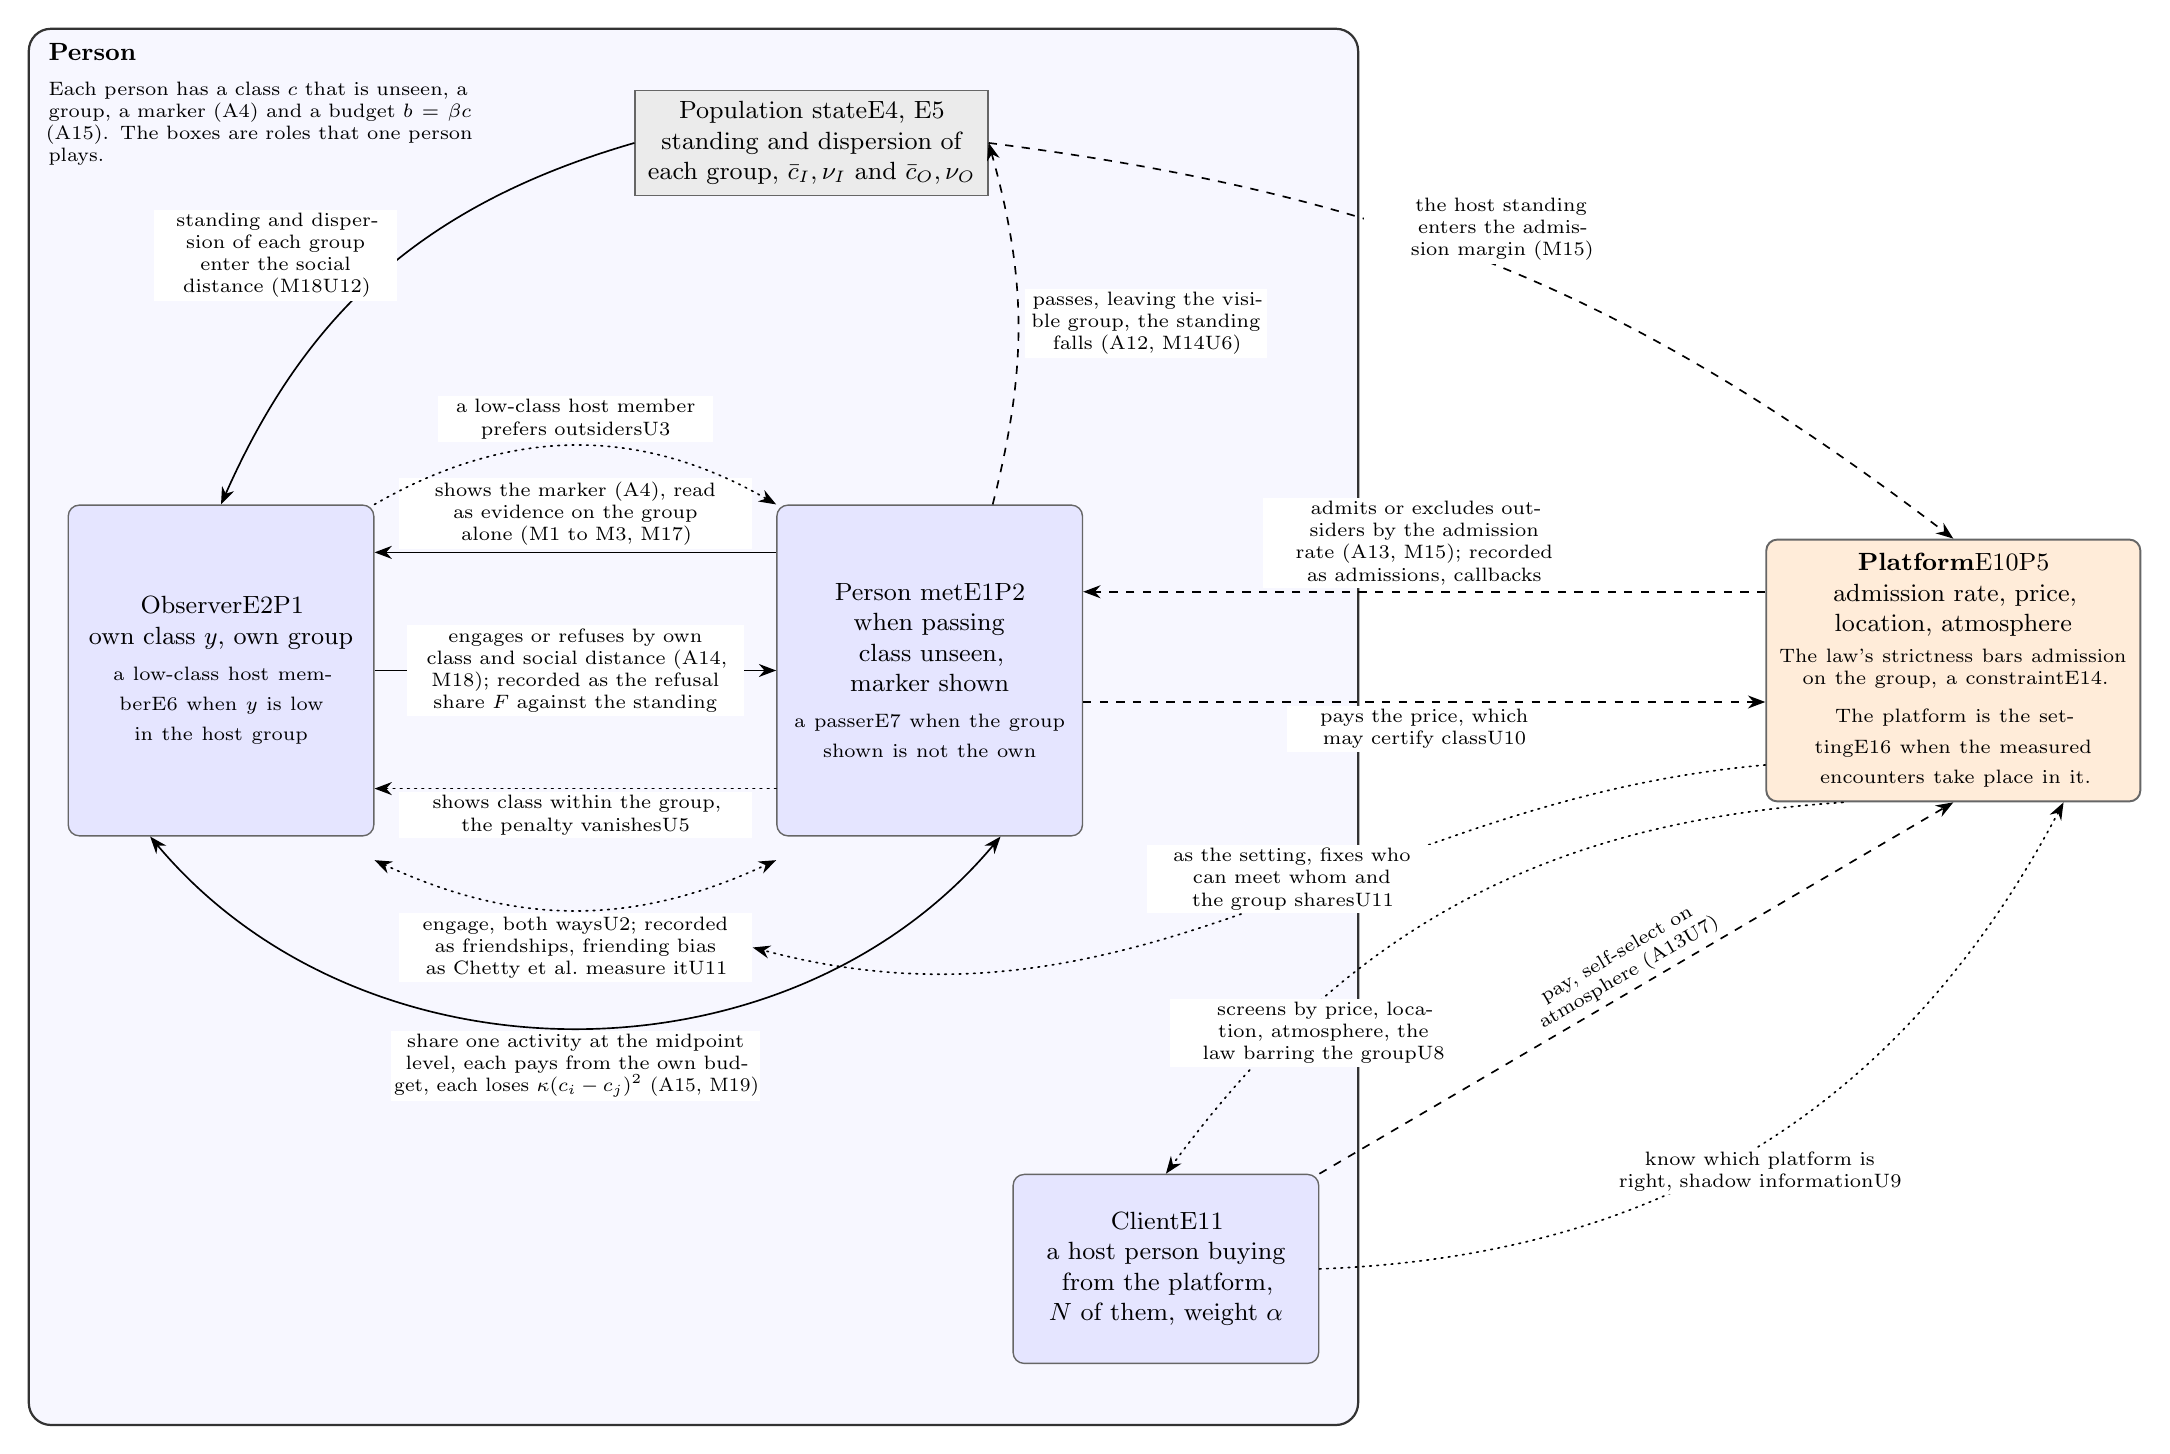
\begin{tikzpicture}[
  >={Stealth[length=2.2mm]},
  every node/.style={font=\small},
  role/.style={draw=black!60, line width=0.5pt, align=center, text width=3.6cm, minimum height=4.2cm, inner sep=4pt, rounded corners=4pt, fill=blue!10},
  pop/.style={draw=black!60, line width=0.5pt, align=center, text width=4.2cm, minimum height=1.2cm, inner sep=4pt, fill=black!8},
  platform/.style={draw=black!60, line width=0.7pt, align=center, text width=4.4cm, minimum height=3.0cm, inner sep=5pt, rounded corners=4pt, fill=orange!15},
  entity/.style={draw=black!80, line width=0.8pt, rounded corners=8pt, inner sep=10pt, fill=blue!3},
  title/.style={font=\small\bfseries, anchor=north west, align=left},
  attr/.style={font=\scriptsize, anchor=north west, align=left, text width=5.6cm},
  lab/.style={font=\scriptsize, align=center, fill=white, inner sep=1.2pt, text width=3.0cm},
  settled/.style={->, line width=0.6pt},
  given/.style={->, line width=0.6pt, dashed},
  open/.style={->, line width=0.6pt, dotted, line cap=round},
  jointsettled/.style={<->, line width=0.6pt},
  jointopen/.style={<->, line width=0.6pt, dotted, line cap=round},
]
% ---------------------------------------------------------------- roles of Person
\node[pop]  (Pop)      at (7.5,9.7) {Population state\eid{E4, E5}\\ standing and dispersion of each group, $\bar c_I,\nu_I$ and $\bar c_O,\nu_O$};
\node[role] (Observer) at (0,3)      {Observer\nodeid{E2}{P1}\\ own class $y$, own group\\[2pt] \scriptsize a low-class host member\eid{E6} when $y$ is low in the host group};
\node[role] (Person)   at (9,3)      {Person met\nodeid{E1}{P2 when passing}\\ class unseen, marker shown\\[2pt] \scriptsize a passer\eid{E7} when the group shown is not the own};
\node[role,minimum height=2.4cm] (Client) at (12,-4.6) {Client\eid{E11}\\ a host person buying from the platform, $N$ of them, weight $\alpha$};

% ---------------------------------------------------------------- the Person entity
\begin{scope}[on background layer]
\node[entity, fit=(Pop)(Observer)(Person)(Client), inner xsep=14pt, inner ysep=22pt] (PersonBox) {};
\end{scope}
\node[title] at ([xshift=4pt, yshift=-2pt]PersonBox.north west) {Person};
\node[attr]  at ([xshift=4pt, yshift=-16pt]PersonBox.north west) {Each person has a class $c$ that is unseen, a group, a marker (A4) and a budget $b=\beta c$ (A15). The boxes are roles that one person plays.};

% ---------------------------------------------------------------- the Platform entity
\node[platform] (Platform) at (22,3) {\textbf{Platform}\nodeid{E10}{P5}\\ admission rate, price, location, atmosphere\\[3pt] \scriptsize The law's strictness bars admission on the group, a constraint\eid{E14}.\\[3pt] \scriptsize The platform is the setting\eid{E16} when the measured encounters take place in it.};

% ---------------------------------------------------------------- person on person, three straight actions
\draw[settled] ([yshift=15mm]Person.west) -- node[lab, pos=0.5, above=1pt, text width=4.4cm] {shows the marker (A4), read as evidence on the group alone (M1 to M3, M17)} ([yshift=15mm]Observer.east);
\draw[settled] (Observer.east) -- node[lab, pos=0.5, text width=4.2cm] {engages or refuses by own class and social distance (A14, M18); recorded as the refusal share $F$ against the standing} (Person.west);
\draw[open]    ([yshift=-15mm]Person.west) -- node[lab, pos=0.5, below=1pt, text width=4.4cm] {shows class within the group, the penalty vanishes\uid{U5}} ([yshift=-15mm]Observer.east);

% ---------------------------------------------------------------- the low-class host member, above
\draw[open]    (Observer.north east) to[bend left=30] node[lab, pos=0.5, above=1pt, text width=3.4cm] {a low-class host member prefers outsiders\uid{U3}} (Person.north west);

% ---------------------------------------------------------------- the population state
\draw[settled] (Pop.west) to[bend right=25] node[lab, pos=0.45, anchor=east, xshift=-2pt, text width=3.0cm] {standing and dispersion of each group enter the social distance (M18\mix{U12})} (Observer.north);
\draw[given]   ([xshift=8mm]Person.north) to[bend right=15] node[lab, pos=0.5, anchor=west, xshift=2pt, text width=3.0cm] {passes, leaving the visible group, the standing falls (A12, M14\mix{U6})} (Pop.east);

% ---------------------------------------------------------------- the two joint actions, below
\draw[jointopen]    ([yshift=-3mm]Observer.south east) to[bend right=25] node[lab, pos=0.5, below=1pt, text width=4.4cm] (PairLab) {engage, both ways\uid{U2}; recorded as friendships, friending bias as Chetty et al.\ measure it\uid{U11}} ([yshift=-3mm]Person.south west);
\draw[jointsettled] ([xshift=-9mm]Observer.south) to[bend right=50] node[lab, pos=0.5, below=1pt, text width=4.6cm] {share one activity at the midpoint level, each pays from the own budget, each loses $\kappa(c_i-c_j)^2$ (A15, M19)} ([xshift=9mm]Person.south);

% ---------------------------------------------------------------- the platform and the person met
\draw[given]   ([yshift=10mm]Platform.west) -- node[lab, pos=0.5, above=1pt, text width=4.0cm] {admits or excludes outsiders by the admission rate (A13, M15); recorded as admissions, callbacks} ([yshift=10mm]Person.east);
\draw[given]   ([yshift=-4mm]Person.east) -- node[lab, pos=0.5, below=1pt, text width=3.4cm] {pays the price, which may certify class\uid{U10}} ([yshift=-4mm]Platform.west);

% ---------------------------------------------------------------- the platform as the setting
\draw[open]    ([yshift=-12mm]Platform.west) to[out=185, in=-15] (PairLab.east);
\node[lab, text width=3.6cm] at (13.6,0.35) {as the setting, fixes who can meet whom and the group shares\uid{U11}};

% ---------------------------------------------------------------- the population state and the platform
\draw[given]   (Pop.east) to[bend left=15] node[lab, pos=0.5, above=1pt, text width=3.4cm] {the host standing enters the admission margin (M15)} (Platform.north);

% ---------------------------------------------------------------- the clients and the platform
\draw[given]   (Client.north east) -- node[lab, pos=0.5, sloped, above=1pt, text width=3.2cm] {pay, self-select on atmosphere (A13\mix{U7})} (Platform.south);
\draw[open]    (Client.east) to[bend right=30] node[lab, pos=0.5, below=1pt, text width=3.6cm] {know which platform is right, shadow information\uid{U9}} ([xshift=14mm]Platform.south);
\draw[open]    ([xshift=-14mm]Platform.south) to[bend right=25] (Client.north);
\node[lab, text width=3.8cm] at (14.0,-1.6) {screens by price, location, atmosphere, the law barring the group\uid{U8}};
\end{tikzpicture}
}
\caption{The model as a graph of two entities, the person and the platform.
The boxes inside the person are roles. An arrow is an action of one role on
another, labelled by the rows that settle the action, and a double arrow is
an action that two roles take together. Solid arrows are settled by model
rows, dashed arrows are rules or inputs taken as given, and dotted arrows
are open. ``Recorded as'' marks an action that reaches the data.}
\label{fig:ledger}
\end{figure}
\end{landscape}


\subsection{Assumptions}

Table~\ref{tab:assumptions} lists the assumptions the model rows rest on, each
with a reading in plain English, the rows that use it and the reason it is
made. The plain-English reading uses no symbols and names each object by its
name in the measurement map. Every symbol in the table has
exactly one row in the measurement map (\texttt{MEASUREMENT\_MAP.tex}), which
says whether the object is an input, an internal object or an output, what
it stands for in the world, whether it is directly observed, and how it is
obtained. Appendix~\ref{app:scope} gives the longer reasons.

\footnotesize
\begin{longtable}{@{}P{0.7cm}P{3.5cm}P{4.2cm}P{2.0cm}P{1.5cm}P{3.3cm}@{}}
\caption{Assumptions of the model.}
\label{tab:assumptions}\\
\toprule
\textbf{ID} & \textbf{Assumption} & \textbf{In plain English} & \textbf{Symbols} & \textbf{Model rows} & \textbf{Reason} \\
\midrule
\endfirsthead
\toprule
\textbf{ID} & \textbf{Assumption} & \textbf{In plain English} & \textbf{Symbols} & \textbf{Model rows} & \textbf{Reason} \\
\midrule
\endhead
\bottomrule
\endfoot
\arow{A1}{Class takes finitely many values $c\in\mathcal{C}$.}
  {A person's class is one of a finite list of values.}
  {$c$, $\mathcal{C}$}{M1, M2, M3, M18}
  {The Lean statements range over a finite set. The predecessor's class in
  $[0,1]$ is outside the rows (Appendix~\ref{app:scope}, Class space).}
\arow{A2}{Class is not seen at the encounter. The observer sees a marker $m$,
  which indicates one of finitely many groups $g\in\mathcal{G}$. The person
  does not acquire the marker by choice, and can suppress it only by passing
  (A12).}
  {The observer cannot see a person's class at the encounter and sees only a
  marker, which is evidence about the person's group. There are finitely
  many groups. The person carries the marker without choosing it, and can
  hide it only by passing, as A12 describes.}
  {$m$, $g$, $\mathcal{G}$}{M1, M2, M3}
  {The premise of the question. That the marker is not acquired by choice
  separates the model from signalling, where the informed person chooses
  the signal at a cost that varies with the hidden type (L17). Akerlof makes
  dialect a choice that tracks whom one meets (L40), so the premise is an
  assumption and not a result.}
\arow{A3}{The observer revises the prior $\pi_g(c)$ and the group weights
  $q(g)$ by Bayes' rule alone, giving the posterior $\pi'_g(c)$, the
  posterior on group $q'(g)$ and the posterior on class $P(c\mid m)$.}
  {The observer starts from a prior on class within each group and from
  group weights. On reading the marker the observer updates both by Bayes'
  rule, through the likelihood of the marker, and by no other rule. The
  results are the posterior within each group, the posterior on group and
  the posterior on class.}
  {$\pi_g(c)$, $\ell_g(c)$, $q(g)$, $\pi'_g(c)$, $q'(g)$, $P(c\mid m)$}
  {M1, M2, M3, M17}
  {The author's choice of 14 October 2026 (Appendix~\ref{app:scope}, The
  updating rule).}
\arow{A4}{Group sufficiency. Within a group the marker's likelihood does not
  depend on class, $\ell_g(c)=Z_g$ for every $c$.}
  {Once the group is known, the marker says nothing more about class. Within
  each group the likelihood of the marker is one constant likelihood for
  every class, and so equals the marginal.
  Lean, \lean{Assumptions.marginal\_of\_flat}.}
  {$\ell_g(c)$, $Z_g$, $\lambda_g$}{M1, M2, M3}
  {The predecessor's assumption. M1 shows its likelihood and posterior forms
  agree under a prior with full support (Appendix~\ref{app:scope}, Group
  sufficiency).}
\arow{A12}{A group is a finite set of people $V$, each with a class $c$. A
  member passes, leaving the visible group, when the passing gain
  $\mathrm{gain}(c)$ is at least the passing cost $\mathrm{cost}(c)$, and the
  passers are $P$.}
  {A group is a finite set of group members, each with a class. A member
  passes, suppressing the marker and leaving the visible group, when the
  passing gain at the member's class is at least the passing cost. The
  members who pass are the passers.}
  {$V$, $c$, $P$, $\mathrm{gain}$, $\mathrm{cost}$}{M14}
  {The predecessor's passing appendix. The gain and the cost are not derived
  (Appendix~\ref{app:scope}, Passing).}
\arow{A13}{A platform admits a share $\sigma$ of outsider applicants to a room
  of $|A|$ attendees, with $N$ host clients, objective weight $\alpha$ and
  willingness to pay $W$. Its profit is $\Pi(\sigma)=\sigma\,\mathrm{marg}$,
  linear in $\sigma$, with the admission margin $\mathrm{marg}$.}
  {A platform sets the admission rate of outsider members into a room of a
  given room size. Its host clients weigh objective quality by the objective
  weight, and an admitted outsider member pays the willingness to pay.
  Platform profit is the admission rate times the admission margin, so it is
  linear in the admission rate.}
  {$\sigma$, $|A|$, $N$, $\alpha$, $W$, $\Pi$, $\mathrm{marg}$}{M15, M20}
  {The predecessor's first-order condition, taken as a definition
  (Appendix~\ref{app:scope}, The platform channel).}
\arow{A14}{The observer of own class $y$ values engagement with a person of
  class $c$ at $v-\kappa\,(c-y)^2$ against the outside option $\bar u$, and
  engages when the social distance $E$ under the posterior on group is at
  most the engagement threshold $\bar d=(v-\bar u)/\kappa$. The observers
  form a finite set $J$. Group $g$ has standing $\bar c_g$ and dispersion
  $\nu_g$ under its prior.}
  {An observer of a given own class values engaging with a person of a given
  class at the baseline value less the sensitivity times the squared
  distance between the two classes, and declines for the outside option. The
  observer engages when the social distance, taken under the posterior on
  group, is at most the engagement threshold, which is the baseline value
  less the outside option, divided by the sensitivity. The observers are
  finitely many. Each group has a standing and a dispersion under its prior.
  Lean, \lean{Engagement.engages\_iff}.}
  {$c$, $y$, $v$, $\kappa$, $\bar u$, $E$, $\bar d$, $J$, $\bar c$, $\nu_g$}
  {M18}
  {The predecessor's engagement rule, its equations (utility) and
  (threshold). The quadratic loss in the economic distance is the form
  Akerlof sets aside as a special case of a benefit that falls with social
  distance (L32). The quadratic form and the sensitivity are derived in M19
  from A15, and what A14 adds is that the observer takes the expectation
  under the posterior on group and that the observers are finitely many
  (Appendix~\ref{app:scope}, The engagement decision).}
\arow{A15}{Class $c$ affords the budget $b=\beta c$ with $\beta>0$. A pair
  that engages shares one activity at one level $p$, which each pays from
  the own budget, leaving private consumption $b-p$. The payoff from the
  level is $\gamma p-\tfrac{h}{2}p^2+(b-p)-\tfrac{a}{2}(b-p)^2$ with
  $a>0$ and $h>0$. Budgets are separate. The pair sets the level that
  minimises the sum of the two losses from the two ideal levels. Engaging
  adds the baseline value $v$ to the payoff from the shared level, and
  declining yields the outside option $\bar u$ with the ideal level alone.}
  {A person's class fixes the budget, in proportion, through the budget
  slope. A pair that engages shares one activity at one activity level,
  each pays for that level from the own budget, and the rest of the budget
  is private consumption. The payoff from the activity level is the
  activity value times the level, less the activity curvature times the
  squared level over two, plus private consumption, less the private
  curvature times squared private consumption over two, with both
  curvatures positive. Budgets are not pooled. The pair chooses the
  activity level that minimises the sum of the two losses against the two
  ideal levels. Engaging adds the baseline value to the payoff from the
  shared level, and declining yields the outside option with the ideal
  level alone. Lean, \lean{Budget.payoff\_eq}.}
  {$c$, $b$, $\beta$, $p$, $\gamma$, $h$, $a$, $v$, $\bar u$}
  {M19, M20}
  {The author's account of budget compatibility as the micro-foundation of
  class homophily, with the quadratic payoff chosen so that the loss, the
  compromise and the sensitivity have closed forms. The general concave
  case carries only the monotonicity of the ideal level (M19 (i)).}
\arow{A16}{For row M21 only, engaging with a person at economic distance $d$
  is worth the benefit of contact $\Phi(d)$, which does not rise in $d$ for
  $d\ge0$. The form of A14 is $\Phi(d)=v-\kappa d^2$.}
  {For row M21 only, engaging with a person is worth a benefit of contact
  that depends on nothing but the economic distance between the two, and that
  does not rise as the economic distance grows. The engagement utility of A14
  is the case where the benefit is the baseline value less the sensitivity
  times the squared economic distance.
  Lean, \lean{Robustness.quadratic\_antitone}.}
  {$\Phi$, $d$, $v$, $\kappa$}{M21}
  {Pass 3 of the work on the engagement utility, 17 October 2026. The other
  rows use A14. A16 is what M21 needs, and both the quadratic loss and the
  benefit of Akerlof (L33) satisfy it (M21 (iii)).}
\arow{A17}{For row M22 only, the activity payoff $\Psi(p,b)$ is concave in
  the level $p$ for each budget $b$, and maximised at the ideal level
  $p^*(b)$, which does not fall in $b$. A person of budget $b$ with a
  partner of budget $b'$ shares the level $(1-\omega)\,p^*(b)+\omega\,p^*(b')$
  for a fixed compromise weight $\omega\in[0,1]$.}
  {For row M22 only, the activity payoff from a level of the shared
  activity, given a budget, is concave in the activity level and is highest
  at the ideal level, which does not fall as the budget rises. A pair shares
  the compromise level that puts the compromise weight on the partner's
  ideal level and the rest on the own. Lean,
  \lean{Budget.loss\_rises\_above}.}
  {$\Psi$, $p$, $b$, $p^*$, $\omega$}{M22}
  {Row M19 (i) gives the ideal level that does not fall in the budget for
  any concave private utility, and A15's quadratic payoff is concave in the
  level (M22). A17 drops the quadratic form and keeps the compromise rule,
  which is assumed and not derived from bargaining.}
\end{longtable}
\normalsize

\subsection{Results}

\footnotesize
\begin{longtable}{@{}P{0.8cm}P{3.8cm}P{6.3cm}P{3.7cm}P{1.1cm}@{}}
\caption{Results of the model, each with its statement and the Lean theorems
that check it.}\\
\toprule
\textbf{ID} & \textbf{Claim} & \textbf{Statement} & \textbf{Lean} & \textbf{Proof} \\
\midrule
\endfirsthead
\toprule
\textbf{ID} & \textbf{Claim} & \textbf{Statement} & \textbf{Lean} & \textbf{Proof} \\
\midrule
\endhead
\bottomrule
\endfoot
\mrow{M1}{A marker whose likelihood does not depend on class leaves the
  Bayesian posterior on class equal to the prior. Under a prior that gives
  every class positive probability, the converse holds, so the two forms of
  group sufficiency are equivalent.}
  {$\mathcal{C}$ finite, $\sum_{c}\pi_g(c)=1$,
  $Z_g=\sum_{c'}\ell_g(c')\,\pi_g(c')$,
  $\pi'_g(c)=\ell_g(c)\,\pi_g(c)/Z_g$.
  (i) If $\ell_g(c)=\lambda_g\neq0$ for every $c$, then $\pi'_g=\pi_g$.
  (ii) If $\pi_g(c)>0$ for every $c$, $Z_g\neq0$ and $\pi'_g=\pi_g$, then
  $\ell_g(c)=Z_g$ for every $c$.
  Neither hypothesis can be dropped.}
  {Sufficiency.posterior_eq_prior_of_flat, Sufficiency.flat_of_posterior_eq_prior, Sufficiency.control_flat_needed, Sufficiency.control_support_needed}
\mrow{M2}{Under group sufficiency, the Bayesian posterior on class is the
  within-group class distributions mixed by the Bayesian posterior on group.}
  {$\mathcal{G}$, $\mathcal{C}$ finite, $\sum_c\pi_g(c)=1$ and
  $\ell_g(c)=\lambda_g$ for every $g$ and $c$. Then
  $P(c\mid m)=\sum_g\pi_g(c)\,q'(g)$ for every $c$.
  It fails without $\ell_g(c)=\lambda_g$, and without
  $\sum_c\pi_g(c)=1$.}
  {ClassPosterior.bayes_class_eq_mixture, ClassPosterior.control_sufficiency_needed, ClassPosterior.control_normalised_needed}
\mrow{M3}{Under a prior that gives every group positive weight, any weights
  on the groups are the Bayesian posterior on group, for a marker likelihood
  that depends on group alone. The posterior on class is then the mixture by
  those weights.}
  {$q(g)>0$, $\sum_g w(g)=1$, $\sum_c\pi_g(c)=1$, $\xi\neq0$ and
  $\ell_g(c)=\xi\,w(g)/q(g)$. Then $q'=w$ and
  $P(c\mid m)=\sum_g\pi_g(c)\,w(g)$. If also $0<\xi\le q(g)$ and
  $0\le w(g)\le1$, then $0\le\ell_g(c)\le1$.
  It fails without $q(g)>0$, since $q=(1,0)$ gives $q'(1)=0$ for every
  $\ell$.}
  {ClassPosterior.bayes_group_of_ratio, ClassPosterior.bayes_class_of_ratio, ClassPosterior.ratioLik_mem_unit, ClassPosterior.control_prior_support_needed}
\mrow{M14}{If the members who leave the visible group are those above every
  member who stays, the visible mean falls, strictly when some leaver is
  above some stayer. A passing cost that does not rise in class and a benefit
  that does not fall in it make the leavers such a set. Under a
  discrimination-rate function that does not rise in standing, the rate
  against those who stay does not fall.}
  {People $V$ finite, classes $c_i$, passers $P\subseteq V$, with $P$ and
  $V\setminus P$ non-empty.
  (i) If $c_j\le c_i$ for every $i\in P$ and $j\in V\setminus P$, then
  $\bar c(V\setminus P)\le\bar c(V)$, and $<$ if some $c_j<c_i$.
  (ii) If $\mathrm{gain}$ is non-decreasing and $\mathrm{cost}$ non-increasing, then
  $\mathrm{cost}(x)\le\mathrm{gain}(x)$ and $x\le y$ give $\mathrm{cost}(y)\le\mathrm{gain}(y)$.
  (iii) If $F$ is non-increasing, $s_g\ge0$ and $\bar c'\le\bar c$, then
  $s_gF(\bar c)\le s_gF(\bar c')$.
  (i) fails without the ordering, since classes $(0,1)$ with the class-$0$
  member leaving give a visible mean of $1$ against $\tfrac12$.}
  {Passing.cross, Passing.mean_sdiff_le, Passing.mean_sdiff_lt, Passing.upper_set_of_threshold, Passing.rate_rises, Passing.control_ordering_needed}
\mrow{M15}{With the predecessor's admission objective, linear in the
  admission rate, the platform excludes the outsider group exactly when an
  admittee's willingness to pay falls short of the composition externality,
  which is exactly when the outsider's standing is below the admission
  threshold.}
  {$\mathrm{marg}=W+N(1-\alpha)(\bar c_O-\bar c_I)/|A|$, $\Pi(\sigma)=\sigma\,\mathrm{marg}$,
  $c_E=\bar c_I-W|A|/(N(1-\alpha))$.
  (i) $|A|>0$. $\mathrm{marg}<0\iff W|A|<N(1-\alpha)(\bar c_I-\bar c_O)$, and
  with $N(1-\alpha)>0$, $\iff\bar c_O<c_E$.
  (ii) $\mathrm{marg}<0$ and $\sigma>0$ give $\Pi(\sigma)<\Pi(0)$.
  (ii) fails with $\mathrm{marg}>0$, where $\Pi(1)>\Pi(0)$.}
  {Platform.marg_neg_iff, Platform.marg_neg_iff_below, Platform.exclude_of_neg, Platform.control_admit_of_pos}
\mrow{M17}{The predecessor's worked example agrees with the rows. Its
  stranger moves from an expected class of $0.50$ to $0.38$, which is the
  mixture of M2 and M3.}
  {The mixture of standings $(\tfrac7{10},\tfrac3{10})$ by weights
  $(\tfrac12,\tfrac12)$ is $\tfrac12$, and by $(\tfrac15,\tfrac45)$ is
  $\tfrac{19}{50}$.}
  {Stranger.stranger_example}
\mrow{M18}{An observer engages when the expected squared economic distance is
  at most the engagement threshold. Under the posterior on group that
  distance is the sum over groups of the squared gap to the group's standing
  plus the group's dispersion. Read as the outsider with certainty, the observer
  refuses exactly when the squared gap to the outsider's standing plus its
  dispersion exceeds the threshold. The refusal share among the observers does
  not rise in the standing on the range at or below every observer's class,
  and does not fall on the range at or above every observer's class. With
  two groups, more weight on the outsider raises the social distance
  exactly when the outsider's social distance exceeds the host's.}
  {$\mathcal{G}$, $\mathcal{C}$ finite, $\sum_c\pi_g(c)=1$,
  $E(w,y)=\sum_c\big(\sum_g\pi_g(c)\,w(g)\big)(c-y)^2$,
  $\bar c_g=\sum_c\pi_g(c)\,c$, $\nu_g=\sum_c\pi_g(c)(c-\bar c_g)^2$,
  $\bar d=(v-\bar u)/\kappa$ with $\kappa>0$.
  (i) $E(w,y)=\sum_g w(g)\,[(\bar c_g-y)^2+\nu_g]$.
  (ii) $\bar u\le v-\kappa E\iff E\le\bar d$. With $w=\mathbf 1_O$,
  $E=(\bar c_O-y)^2+\nu_O$, and the observer refuses iff
  $\bar d<(\bar c_O-y)^2+\nu_O$.
  (iii) $F(\bar c)=|\{j\in J:\bar d<(\bar c-y_j)^2+\nu_O\}|/|J|\in[0,1]$.
  If $\bar c\le\bar c'\le y_j$ for every $j\in J$ then $F(\bar c')\le F(\bar c)$,
  and if $y_j\le\bar c\le\bar c'$ for every $j\in J$ then $F(\bar c)\le F(\bar c')$.
  (iv) $(1-s_g)E_I+s_gE_O=E_I+s_g(E_O-E_I)$, which for $s_g\le s_g'$ does not
  fall when $E_I<E_O$ and does not rise when $E_O<E_I$, and $w=(1-s_g,s_g)$
  in (i) gives this mixture.
  (iii) fails off its range, since $J=\{0\}$, $y_0=0$, $\nu_O=0$, $\bar d=1$
  give $F(1)=0$ and $F(2)=1$. (iv) is constant in $s_g$ when $E_I=E_O$.}
  {Engagement.second_moment, Engagement.expDist_decomp, Engagement.expDist_certain, Engagement.engages_iff, Engagement.refusal_iff, Engagement.refusalShare_antitone, Engagement.refusalShare_monotone_above, Engagement.refusalShare_mem, Engagement.control_observer_below, Engagement.salience_slope, Engagement.salience_effect, Engagement.control_equal_distances, Engagement.expDist_two_groups}
\mrow{M19}{Under separate budgets and one shared activity at one level, the
  ideal level does not fall in the budget, for the quadratic payoff and for
  any concave private utility. The level that minimises the sum of the two
  losses is the midpoint of the two ideals, and each side then loses the
  sensitivity times the squared class gap, the same amount on either side.
  The engagement decision against the outside option is the threshold rule
  of A14 with that sensitivity. The compromise lies within the poorer
  partner's budget exactly when the class gap is at most a bound that rises
  in the poorer partner's budget. A linear private utility gives every
  budget the same ideal level and no loss, and pooled budgets give a payoff
  that depends on the sum of the budgets alone.}
  {$V(p,b)=\gamma p-\tfrac{h}{2}p^2+(b-p)-\tfrac{a}{2}(b-p)^2$, $a+h>0$,
  $p^*(b)=(ab+\gamma-1)/(a+h)$, $\bar p=(p^*(b_i)+p^*(b_j))/2$,
  $\kappa=a^2\beta^2/(8(a+h))$.
  (i) $V(p,b)=V(p^*(b),b)-\tfrac{a+h}{2}(p-p^*(b))^2$, so $p^*(b)$ is the
  unique maximiser, and $p^*(b')-p^*(b)=a(b'-b)/(a+h)\ge0$ for $b\le b'$,
  $a\ge0$. For any concave $\varphi$ and any $\psi$, $\varphi(b-p)+\psi(p)$
  has increasing differences in $(p,b)$, and a maximiser at $b$ is at most
  the unique maximiser at $b'\ge b$.
  (ii) $L(p,b)=V(p^*(b),b)-V(p,b)=\tfrac{a+h}{2}(p-p^*(b))^2$, and
  $L(\bar p,b_i)+L(\bar p,b_j)\le L(p,b_i)+L(p,b_j)$ for every $p$, with
  $L(\bar p,b_i)=L(\bar p,b_j)=\tfrac{a^2}{8(a+h)}(b_i-b_j)^2$. At the level
  $(1-\omega)p^*(b_i)+\omega p^*(b_j)$ the losses are
  $\tfrac{a+h}{2}\omega^2$ and $\tfrac{a+h}{2}(1-\omega)^2$ times
  $(p^*(b_i)-p^*(b_j))^2$, equal iff $\omega=\tfrac12$ or the ideals
  coincide.
  (iii) With $b=\beta c$, $v+V(\bar p,b_i)-V(p^*(b_i),b_i)=v-\kappa(c_i-c_j)^2$
  and the same for $j$, $\kappa>0$ for $a\ne0$, $\beta\ne0$, and
  $\bar u\le v-\kappa(c_i-c_j)^2\iff(c_i-c_j)^2\le(v-\bar u)/\kappa$.
  (iv) For $a>0$, $\bar p\le b_j\iff b_i-b_j\le2(hb_j-\gamma+1)/a$, and the
  bound does not fall in $b_j$ for $h>0$.
  Controls. $a=0$ gives $p^*(b)=(\gamma-1)/h$, $L(\bar p,b_i)=0$ and
  $\kappa=0$. Pooling gives $V(p^*(b_i+b_j),b_i+b_j)$, equal for equal sums,
  and $p^*(b_i+b_j)$ does not fall in $b_j$. Under separate budgets
  $v-\kappa(c_i-c_j')^2<v-\kappa(c_i-c_j)^2$ when $(c_i-c_j)^2<(c_i-c_j')^2$.}
  {Budget.payoff_eq, Budget.loss_eq, Budget.ideal_max, Budget.ideal_unique, Budget.ideal_sub, Budget.ideal_mono, Budget.argmax_mono, Budget.payoff_increasing_differences, Budget.concave_four_point, Budget.concave_increasing_differences, Budget.mid_min, Budget.loss_mid, Budget.engagement_utility, Budget.sensitivity_pos, Budget.engage_iff, Budget.weighted_losses, Budget.weighted_equal_iff, Budget.affordable_iff, Budget.bound_mono, Budget.control_linear_private, Budget.control_pooled_gap_free, Budget.control_pooled_level_mono, Budget.control_separate_gap_cost}
\mrow{M20}{The sensitivity does not rise in the activity curvature and does
  not fall in the budget slope, and the engagement threshold does not fall
  as the sensitivity falls. The admission threshold does not rise in the
  willingness to pay, the room size or the objective weight, and does not
  fall in the number of host clients.}
  {(i) $0<a+h$ and $h\le h'$ give $\kappa(a,h',\beta)\le\kappa(a,h,\beta)$.
  (ii) $0\le\beta\le\beta'$ gives $\kappa(a,h,\beta)\le\kappa(a,h,\beta')$.
  (iii) $u\le v$ and $0<\kappa\le\kappa'$ give $(v-u)/\kappa'\le(v-u)/\kappa$.
  (iv) With $0\le W$, $0\le|A|$, $0<N$ and $\alpha<1$, $c_E$ does not rise
  in $W$, in $|A|$ or in $\alpha$, and does not fall in $N$.
  (iii) reverses with $v<u$, and (iv) reverses in $|A|$ with $W<0$.}
  {Implications.sensitivity_antitone_h, Implications.sensitivity_mono_beta, Implications.threshold_antitone, Implications.control_threshold_reverses, Implications.cAdm_antitone_W, Implications.cAdm_antitone_A, Implications.cAdm_mono_n, Implications.cAdm_antitone_alpha, Implications.control_cAdm_negative_W}
\mrow{M21}{For any benefit of contact that does not rise in the class
  distance, a rise in every member's class does not raise refusal among
  observers at or above every member and does not lower it among observers
  at or below every member. When the benefit is concave in distance, a
  mean-preserving widening of a group's classes does not raise the expected
  benefit to any observer. When the benefit is convex, a widening whose
  classes all stay on one side of an observer does not lower the expected
  benefit to that observer, and an observer inside the widening can lose.
  The benefit of A14 is concave, and Akerlof's is convex.}
  {$S$ finite, $p_i\ge0$, classes $x_i$, observers $J$ with classes $y_j$,
  $t\ge0$, $\Phi$ not rising on $[0,\infty)$.
  (i) If $x_i+t\le y_j$ for every $i$ and $j$, then
  $|\{j:\sum_ip_i\Phi(|y_j-x_i-t|)<\bar u\}|\le|\{j:\sum_ip_i\Phi(|y_j-x_i|)<\bar u\}|$,
  and if $y_j\le x_i$ for every $i$ and $j$ the reverse holds.
  (ii) A widening replaces each $x_i$ by classes $z_{ik}$, $k\in K_i$, with
  $q_{ik}\ge0$, $\sum_kq_{ik}=1$ and $\sum_kq_{ik}z_{ik}=x_i$. Concave
  $\Phi$ gives $\sum_ip_i\sum_kq_{ik}\Phi(|y-z_{ik}|)\le\sum_ip_i\Phi(|y-x_i|)$
  for every $y$. Convex $\Phi$ gives the reverse when $z_{ik}\le y$ for all
  $i,k$, and when $y\le z_{ik}$ for all $i,k$. With two members at $D\mp s$
  and $0\le s\le s'\le D$, convex $\Phi$ gives
  $\Phi(D-s)+\Phi(D+s)\le\Phi(D-s')+\Phi(D+s')$, concave $\Phi$ the reverse,
  and $\Phi(s')\le\Phi(s)$ at the centre.
  (iii) $v-\kappa d^2$ is concave and does not rise for $\kappa\ge0$, and
  $(g+d)^{-1}$ is convex and does not rise for $g>0$.
  Between the ends of (i) the sign turns on $\Phi$, and (ii) changes sign
  with the curvature. Convex $(1+d)^{-1}$, one member at $0$ widened to
  $\pm1$, gives the observer at $0$ the benefit $\tfrac12<1$.}
  {Robustness.shift_up_above, Robustness.shift_up_below, Robustness.refusers_above, Robustness.refusers_below, Robustness.control_range_needs_quadratic, Robustness.majorize, Robustness.spread_convex, Robustness.spread_concave, Robustness.spread_at_centre, Robustness.concave_in_class, Robustness.widen_concave, Robustness.convex_in_class_below, Robustness.convex_in_class_above, Robustness.widen_convex_above, Robustness.widen_convex_below, Robustness.control_widen_inside, Robustness.quadratic_concave, Robustness.quadratic_antitone, Robustness.gravity_convex, Robustness.gravity_antitone, Robustness.control_spread_sign}
\mrow{M22}{For any activity payoff concave in the activity level, with an
  ideal level that does not fall in the budget and a fixed compromise
  weight, each side's loss from the shared level does not fall as the
  partner's budget moves away from the own budget, on either side. With the
  budget rising in class, the loss does not fall in the economic distance,
  so the cost of the economic distance does not need the quadratic payoff.
  The quadratic payoff of A15 is a case.}
  {$\Psi(\cdot,b)$ concave on $\mathbb R$, $\Psi(x,b)\le\Psi(p^*(b),b)$ for
  every $x$, $p^*$ non-decreasing, $\omega\ge0$,
  $\bar p_\omega(b_i,b_j)=(1-\omega)p^*(b_i)+\omega p^*(b_j)$.
  (i) $p^*(b)\le p\le q$ or $q\le p\le p^*(b)$ give $\Psi(q,b)\le\Psi(p,b)$.
  (ii) $b_i\le b_j\le b_j'$ give
  $\Psi(\bar p_\omega(b_i,b_j'),b_i)\le\Psi(\bar p_\omega(b_i,b_j),b_i)$, and so
  do $b_j'\le b_j\le b_i$.
  (iii) $0\le\Psi(p^*(b_i),b_i)-\Psi(\bar p_\omega(b_i,b_j),b_i)$.
  (iv) For $a+h\ge0$ the payoff of A15 is concave in $p$.
  (i) fails without concavity, since $-(p^2-2p)^2$ is maximised at $0$ and
  is $-1$ at $1$ and $0$ at $2$.}
  {Budget.concave_loss_right, Budget.concave_loss_left, Budget.general_loss_nonneg, Budget.loss_rises_above, Budget.loss_rises_below, Budget.payoff_concave, Budget.control_concavity_needed}
\end{longtable}
\normalsize

\section{Literature}

\subsection{How the papers read answer the question}

The papers read solve the question in four ways. Each way is a position on
four axes, what each agent decides, what pins the belief the decision takes
as given, whether the signal is chosen, and whether the deciding agent's own
type enters.

Two families keep the signal unchosen. In the first, one agent decides
against the signal and no equilibrium is needed. \citet{Phelps1972} and
\citet{AignerCain1977} have an employer predict productivity from a group
prior and a test score (L4, L8), and \citet{FryerJackson2008} have a
decision maker file encounters seen in full (L13). In the second, each agent
decides against a group's rate, and the rate must equal what the decisions
produce. \citet{FangMoro2010} call that condition a Bayesian Nash
equilibrium and read discrimination in it as a coordination failure (L14,
L15). \citet{KimLoury2014} assume the employer's belief equals the group's
actual rate (L23), and in \citet{CraigFryer2017} the value of a match does
not depend on the chooser's own type (L16).

Two families change what is seen. In the third, the informed person chooses
the signal at a cost or benefit that varies with the hidden type, so the
choice reveals the type. \citet{CorneoJeanne1994} read income from a
purchase whose sole purpose is the message (L17), \citet{CharlesEtAl2007}
have visible spending kept up at the cost of other categories (L11),
\citet{Pesendorfer1995} have the value of a pool depend on the chooser's own
type (L19), and \citet{AustenSmithFryer2003} have a group accept a person
when the posterior on the person's type clears a threshold (L18). In the
fourth, contact is strategic and often needs both sides, and nothing is
hidden. \citet{CurrariniEtAl2008} have no one refused (L20),
\citet{MailathPostlewaite2006} have no asymmetric information (L21),
\citet{Eguia2013} has each agent know the own skill (L22), and
\citet{PeskiSzentes2012} have the employer see the whole type (L9).
\citet{Akerlof1997} makes the value of contact fall with the distance
between social positions that everyone knows, so the chooser's own position matters
and nothing is read from a marker (L34).

The method here stands with the first family on the signal and apart from
all four on the reader. The marker is not acquired by choice (A2), and class
stays hidden behind it, so the posterior on class is the within-group
distributions mixed by the posterior on group (A4, M1 to M3). The marker can
still be shed by choice. A member passes when the passing gain is at least
the passing cost, and with a gain that does not fall and a cost that does
not rise in class the passers stand at or above every member who stays
(A12, M14). The passing rule is a separation by a cost that varies with
type, which the third family uses to reveal the type and which passing uses
to hide it. The observer's
belief does not take the passing rule into account, and M14 carries only
the step from the passers to the visible mean. Akerlof goes further and
makes dialect itself a choice, correlated with membership because people
conform to those they meet (L40), which the first family and this paper
both rule out by assumption. The observer's own class
enters the decision to engage, so the direction of a group's effect on
refusal depends on who the observer is (M18). No family has that in a
reader of a hidden type. In the second the own type enters only the own
investment (L16), in the third it enters the signaller's choice and not the
reader's (L17), and in the fourth it enters with nothing hidden (L21). Two
readers come near, and neither refuses by own class. Pesendorfer's consumer
values a pool by the own type and refuses no one (L19), and Austen-Smith
and Fryer's group accepts on a posterior and has no type of its own (L18).
Two things the families settle are left open here.
Beliefs are not tied to the actual rates, a condition the second and
third families impose (L14, L23), and the mutual consent of the fourth family is
the dotted double arrow of Figure~\ref{fig:ledger}. Whether each result is
new waits on Table~\ref{tab:pending}.

\subsection{The engagement utility}

\subsubsection{The utility, and the two distances}

The utility rests on two distances. The economic distance between two
people is the gap between their classes. No one sees it, and it costs
something, because class affords a budget, and a pair that engages shares
one activity at one activity level that each pays for from the own budget
(A15). The richer person has the costlier ideal level, the pair settles at the
compromise level between the two ideal levels, and each side loses the
sensitivity times the squared economic distance (M19). The social distance
is what the observer makes of the economic distance from the marker, the
expected squared economic distance under the posterior on group, and the
observer engages when the social distance is at most the engagement
threshold (M18). The square is what lets the social distance depend on a
group through two numbers, its standing and its dispersion (M18). Under any
other benefit of contact the observer's expected benefit runs over every
class within the group (M21). The controls of the derivation can be
checked. Pooled budgets, the origin of assortative matching in Mailath and
Postlewaite (L10), remove the loss, and so does a linear private utility
(M19). What is still assumed is the quadratic payoff of A15, one step below
the form it replaces, and the pair's rule of settling at the compromise
level. The loss rising in the economic distance does not need the square,
and holds for any activity payoff concave in the activity level (M22).

\subsubsection{Against the papers read}

The papers read value the other person in three ways. Most put the other
on one scale that every decider shares, an expected productivity, a quality
or an income, so a group that rises is worth more to every decider and the
decider's own type plays no part in the direction (L9, L16, L10). Two let
the decider's own type set how much a higher type is worth, through a
complementarity that each assumes. Pesendorfer's high types value a match
with high types more than low types do (L19), and Eguia's skilled
incumbents value their group's average skill more than the less skilled do
(L36). Akerlof and the engagement utility value the other by the distance
from the decider's own position (L34, A14). Under a shared scale the
decider's own type leaves the value of a rise in a group unchanged, and
under a complementarity the own type changes how much the rise is worth.
Under a distance the own type changes whether the rise brings the group
nearer or takes it further, and that is how the direction of a group's
effect on refusal comes to depend on the observer's own class (M18).

Akerlof's social distance is the distance between positions that everyone
knows, which is the economic distance here with nothing hidden (L34), and
the social distance here, read from a marker, has no counterpart in his
model. His benefit falls in that distance by a gravity formula taken from
the trade literature by convention (L32), Currarini, Jackson and Pin assume
a taste for the own type (L20), and Hitsch, Horta\c{c}su and Ariely enter
the distances squared because their model is not identified with linear
distances (L35), where here the square is derived from the budgets (M19).
Akerlof's benefit and the quadratic loss differ in curvature, and the
dispersion is where the curvature shows. A group's dispersion enters the
value in two of the papers read. Aigner and Cain discount expected
productivity for risk (L8), and Rothschild and White let a college's
benefit fall in the variance of its students' ability (L39). Charles, Hurst
and Roussanov name the variance and leave it out as hard to tell from the
mean (L37), and Eguia names the whole distribution of skills and keeps the
average (L38). The other papers read value a group by its mean alone. Here
the dispersion enters because the social distance is the squared gap to the
standing plus the dispersion (M18). The quadratic loss is concave in
distance, so any mean-preserving widening of a group lowers the expected
benefit to every observer. Akerlof's benefit is convex, so a widening that
stays on one side of an observer does not lower the benefit to that
observer, and an observer inside the widening can lose (M21, L33).

\subsubsection{Three levels of dependence}

The conclusions divide by what each needs of the benefit of contact, and
Table~\ref{tab:levels} sorts them. The first level needs only that the
benefit falls in the economic distance, or needs no utility at all. The
second needs its curvature. The third needs the square. The platform's
admission objective is not the engagement utility (A13), so M15, C11 and I5
stand outside the three levels.

\footnotesize
\begin{longtable}{@{}P{2.3cm}P{4.6cm}P{3.6cm}P{5.5cm}@{}}
\caption{What each result needs of the benefit of contact.}
\label{tab:levels}\\
\toprule
\textbf{Level} & \textbf{What the benefit must satisfy} & \textbf{Rows} &
\textbf{Conclusions and implications} \\
\midrule
\endfirsthead
\toprule
\textbf{Level} & \textbf{What the benefit must satisfy} & \textbf{Rows} &
\textbf{Conclusions and implications} \\
\midrule
\endhead
\bottomrule
\endfoot
Any benefit, or none & It falls in the economic distance, or no utility
  enters the row. For the budgets, an activity payoff concave in the level &
  \rowref{M1, M2, M3, M17}; \rowref{M14} (i), (ii); \rowref{M21} (i);
  \rowref{M22} & C1, C19, C20. C10, given a rate that does not rise in
  the standing. C25, the direction at the two ends of the class range. C24,
  the cost of the economic distance from separate budgets. \\
  \addlinespace
The curvature & It is concave, or convex, in the economic distance &
  \rowref{M21} (ii) & C25, the sign of the dispersion. K9. I1, which helps
  every observer under a concave benefit and only observers outside the
  widening under a convex one. \\
  \addlinespace
The square & It is the baseline value less the sensitivity times the
  squared economic distance & \rowref{M18, M19, M20} & C21, C23. K7, K8. I2,
  whose range is observers at or above the standing. I3, whose sensitivity
  is the closed form of M19. The social distance as standing plus
  dispersion. \\
\end{longtable}
\normalsize

\subsection{Papers read}

\footnotesize
\begin{longtable}{@{}P{0.8cm}P{2.2cm}P{3.5cm}P{5.5cm}P{1.3cm}P{1.9cm}@{}}
\caption{Papers read, with the passage each row relies on.}\\
\toprule
\textbf{ID} & \textbf{Paper} & \textbf{What we rely on} & \textbf{Quote} &
\textbf{Page} & \textbf{Rows} \\
\midrule
\endfirsthead
\toprule
\textbf{ID} & \textbf{Paper} & \textbf{What we rely on} & \textbf{Quote} &
\textbf{Page} & \textbf{Rows} \\
\midrule
\endhead
\bottomrule
\endfoot
\lrow{L4}{Phelps1972}{The employer combines a group prior with a test
  score, weighting each inversely to its error variance. The group enters as
  a prior about the individual, as in M1 to M3. The parallel ends at the
  evidence. His test score is evidence about the individual, whereas the
  marker here is evidence about the group alone (M1).}{The weights applied to the test information and the skin
  color information are inversely related to the variances of the respective
  disturbance terms corresponding to them.}{660}{M1, C19}
\lrow{L8}{AignerCain1977}{The employer chooses the group that maximises
  expected productivity discounted for risk, so a group's conditional
  variance is penalised in its own right. The dispersion term of M18 is this
  penalty in a contact setting, with economic distance in place of
  productivity. The parallel ends at the observer, whose own class enters
  M18 and plays no part in the employer's choice.}{an employer with this
  utility function will attempt to hire from the group of workers that
  maximizes expected productivity, q, discounted for risk}{8}{M18}
\lrow{L9}{PeskiSzentes2012}{Statistical discrimination gives a signal the
  same value for every employer, so a mutual bias between colours cannot
  come from it. In M18 the posterior is the same for every observer and the
  decision it supports is not, since the squared gap to a group's standing
  depends on the observer's own class. The parallel ends there.}{Such a
  phenomenon is inconsistent with statistical discrimination because the
  signal value of colour must be the same for any employer, regardless of
  his own colour.}{5}{M18, C21}
\lrow{L10}{MailathPostlewaite2006}{Assortative matching on income comes from
  joint consumption, under which everyone prefers a richer partner and a
  preference over partners is vertical. In M19 the budgets are separate,
  the payoff depends on the gap between the two budgets and not on the
  partner's budget alone, and the pooled payoff is the control that depends
  on the sum of the budgets and not on the gap.}{The critical implication
  of the assumption that consumption is joint is that agents prefer richer
  partners, all else equal.}{6}{M19, C23}
\lrow{L11}{CharlesEtAl2007}{At equal total spending, the budget is allocated
  across categories, and visible spending is drawn from the other
  categories. The budget of M19 is split between one shared activity and
  private consumption in the same way, and the richer person's larger
  budget is what makes the costlier activity level the richer person's
  ideal.}{Blacks consume less than Whites in essentially every other
  expenditure category (aside from housing) to maintain higher visible
  consumption.}{4}{M19}
\lrow{L12}{HitschEtAl2006}{In dating data a user's own income changes the
  valuation of a partner's income only slightly, so the preference over a
  partner's income is vertical there. The squared gap of M19 is the cost of
  sharing an activity at one level, which is a cost in the gap and not a
  valuation of the partner's budget, and the dating evidence limits how far
  M19 can be read as a preference over partners.}{own income matters only
  slightly in the evaluation of a partner’s earnings.}{28}{M19}
\lrow{L13}{FryerJackson2008}{The decision maker sees every attribute and
  stores them coarsely, so nothing is unseen. Here class is unseen behind
  the marker (A2), and the observer's belief, not the observer's memory,
  carries the group.}{it results from an inherent bias against minority
  interactions in the process of categorization of human memory, even when
  qualifications are fully observable.}{7}{M1}
\lrow{L14}{FangMoro2010}{The survey's definition of the equilibrium of the
  models with inter-group interaction. Each player optimises against the
  others' strategies, and the group's rate must equal what those strategies
  produce. The observer of M18 optimises against a prior, and no such
  condition is imposed.}{A Bayesian
  Nash equilibrium of the game is a list including the workers’ skill
  investment decision [...] such that every player optimizes against
  other}{30}{M18}
\lrow{L15}{FangMoro2010}{In the models of Coate and Loury's kind,
  discrimination is a choice between equilibria. Refusal in M18 comes from
  the economic distance under one belief, and no coordination is
  involved.}{Discrimination in this model can be viewed as a coordination
  failure.}{18}{M18}
\lrow{L16}{CraigFryer2017}{Neither side's value of a match depends on the
  own investment, so the preference over partners is vertical. In M18 the
  observer's own class sets the distance, and with it the direction of the
  group's effect.}{further assume that the benefit to workers (resp. firms)
  from being matched to a good firm (resp. worker) is independent of their
  own investment decision.}{42}{M18}
\lrow{L17}{CorneoJeanne1994}{The signal is a purchase chosen by the informed
  person at a cost that falls in income, so the choice reveals rank. The
  marker here is not chosen (A4), and what is read from it is the group
  alone (M1).}{Its sole purpose is to send a message about the individual's
  rank in the income hierarchy.}{6}{M1}
\lrow{L18}{AustenSmithFryer2003}{The group accepts a person when the
  posterior on the person's type clears a threshold, the nearest rule in
  the papers read to the engagement threshold of M18. The group has no type
  of its own, so the acceptance cannot depend on the reader's own class, and
  the person chooses the signal by schooling.}{the belief the group must
  hold regarding the individual's type, [...] must be no smaller than the
  quantity}{15}{M18}
\lrow{L19}{Pesendorfer1995}{The value of a pool depends on the chooser's own
  type, the nearest the papers read come to the own class of M18. The
  chooser buys a design, is matched at random within its pool and refuses
  no one.}{types value a match with high types more}{5}{M18}
\lrow{L20}{CurrariniEtAl2008}{Homophily arises with no one refused, from a
  taste for the own type and a meeting bias that are assumed. In M18
  refusal is the decision, and in M19 the homophily is derived from
  separate budgets.}{We remark that in this model the homophily and
  segregation of types that results, never involves an individual being
  rejected as a friend by another individual.}{15}{M18, M19}
\lrow{L21}{MailathPostlewaite2006}{Nothing is unseen in the matching, and
  income is seen when people match. Here class is unseen (A2) and read from
  the marker (M1).}{Social assets play an entirely [...] role in our model
  as there is no asymmetric information, hence no role for
  signalling.}{30}{M1}
\lrow{L22}{Eguia2013}{Each agent knows the own skill, so nothing is inferred
  about a person from the group. The incumbents set one barrier for the
  whole group, and no reader forms a posterior.}{Since each agent knows her
  own skill, in equilibrium no agent is misallocated.}{13}{M1}
\lrow{L23}{KimLoury2014}{The believed rate equals the group's actual rate by
  assumption. Here the standing is the mean of the observer's prior (A14),
  and no consistency condition is imposed.}{We assume that employers have
  correct beliefs at each date about human capital acquisition within each
  population group.}{11}{M18}
\lrow{L24}{Pesendorfer1995}{A seller's value is the average type of its
  clientele, so a sign that certifies class loses value as those below buy
  it. The dispersion that I1 narrows widens again as the sign is copied, and
  the sign is replaced.}{are mostly low types will be less attractive
  to}{16}{M18}
\lrow{L25}{ChettyEtAl2022b}{Friending bias rises with racial diversity
  across schools. Mixing a setting raises exposure and the bias within it,
  so the composition that I2 would set is not the composition the standing
  is read from.}{Friending bias is also higher in more racially diverse
  schools, as measured by a Herfindahl–Hirschman index (Extended Data Fig.
  1e) or the share of white students in the school (Extended Data Fig.
  1f).}{9}{M18}
\lrow{L26}{ChettyEtAl2022b}{A rule neutral on race that assigned students
  to learning communities produced separated concentrations by race, the
  sorting within a setting that undoes a pairing by standing.}{causing
  implicit segregation, resulting in student learning communities with
  separated concentrations of white students and students of
  color}{12}{M18}
\lrow{L27}{ChettyEtAl2022b}{A costly sub-venue on campus is offered as a
  source of friending bias. The richer set their own level there, which is
  the sorting between settings that limits I3.}{feature significant Greek
  life, where the high costs of fraternity and sorority dues may generate
  friending bias on campus}{10}{M19}
\lrow{L28}{DahisEtAl2019}{Passing paid. A policy that lowers the passing
  gain keeps the better-off visible at the cost of that return, the
  tension in I4.}{Column (1) shows that an individual who has passed for
  white earned a higher income}{35}{M14}
\lrow{L29}{KimLoury2012}{The able choose the group with the greater return
  to skill, not the group with the better reputation. Keeping the
  better-off visible by the passing gain does not hold the able when the
  return to skill is elsewhere.}{The disproportionately more talented
  workers, whose human capital investment costs (c) are relatively lower,
  choose the 'affect' that corresponds to the greater return to human
  capital investment}{14}{M14}
\lrow{L30}{EdelmanEtAl2017}{A platform rule that makes sellers pre-commit
  to accept every buyer removes the screen. The admission the rule forces
  is the admission I5 reaches by the margin, and the screen moves to the
  host's room.}{sellers effectively pre-commit to accept all buyers
  regardless of race or ethnicity.}{4}{M15}
\lrow{L31}{LaouenanRathelot2022}{Statistical discrimination is larger in
  shared flats than in entire ones. The host's own room is where the screen
  goes once the platform admits everyone.}{Our analysis shows that shared
  flats tend to have higher statistical discrimination than entire
  flats.}{18}{M15}
\lrow{L32}{Akerlof1997}{The quadratic loss in distance, under which the
  marginal loss vanishes at zero distance, is the case Akerlof sets aside.
  A14 uses it, and M19 derives it from separate budgets and one shared
  activity, where Akerlof takes his form of the benefit from the trade
  literature by convention.}{I have considered utility functions of this
  sort-with the marginal utility of decreased distance vanishing at zero-to
  be a special case.}{7}{M18, M19}
\lrow{L33}{Akerlof1997}{The benefit falls in distance toward zero and is
  convex, so a wider dispersion helps an observer far from the group
  (\path{Akerlof1997.contrast_spread_helps_distant}), and an observer above
  the standing but below some members can lose as the group rises
  (\path{Akerlof1997.control_benefit_range_differs}). The dispersion term and
  the ranges of M18 belong to the quadratic loss. The direction for
  observers beyond every member survives any benefit that falls in distance
  (\path{Akerlof1997.contrast_shift_up_above}).}{as either the initial or
  the acquired social distance between a pair of individuals increases, the
  value of social exchange between them declines asymptotically toward
  zero.}{9}{M18}
\lrow{L34}{Akerlof1997}{The value of contact depends on the chooser's own
  position, with every position known. The dependence of M18 on the
  observer's own class runs through a posterior on group read from a marker,
  which Akerlof's model does not have.}{since person 3 does not much value
  trade with persons 1 or 2 since she is initially so socially distant from
  both of them, she chooses a value of x that is close to the economic
  optimum value of b/2a.}{10}{M18, C22}
\lrow{L35}{HitschEtAl2006}{The distances between the two users' attributes
  enter the utility squared, because the model is not identified when they
  enter linearly. The square is a choice for identification there, where
  M19 derives it from separate budgets and one shared activity.}{We instead
  estimate the model with quadratic differences}{25}{M19}
\lrow{L36}{Eguia2013}{The value of the group's average skill rises in the
  incumbent's own skill, by an assumed complementarity. The own type sets
  how much a more skilled group is worth, and a more skilled group is worth
  more to every member. In M18 the observer's own class sets whether a rise
  brings the group nearer.}{highly skilled individuals, who appreciate their
  group’s average skill more than less skilled individuals}{12}{M18}
\lrow{L37}{CharlesEtAl2007}{The variance of group income is named as a
  determinant of status and left out of the model. In M18 the dispersion enters
  every observer's social distance.}{In general, equilibrium status can
  also depend on higher moments of the income distribution, such as the
  variance.}{22}{M18, M21}
\lrow{L38}{Eguia2013}{The whole distribution of skills in a group is named
  as an extension, and the value of a group keeps its average skill alone.
  In M18 the dispersion enters every observer's social distance.}{assuming
  that v depends on the whole distribution of skills in group J, and not
  only on the average}{14}{M18, M21}
\lrow{L39}{RothschildWhite1993}{The benefit of a college falls in the
  variance of its students' ability, as a cost of teaching that is supposed
  rather than derived. The dispersion term of M18 penalises the dispersion through
  the quadratic loss, and its sign follows the curvature of the benefit of
  contact (M21).}{a decreasing function of the variance of
  ability}{10}{M18, M21}
\lrow{L40}{Akerlof1997}{Dialect is a choice variable, and conformity to
  those one interacts with makes it correlate with membership. A2 takes the
  marker as carried without choice, and A4 takes its likelihood within a
  group as flat. Akerlof's account is a reason the marker carries group
  information, and also a reason it may not be exogenous, which no row of
  this paper addresses.}{x could represent pronunciation or language, with
  the model showing theoretically why there might be a correlation between a
  choice variable, such as dialect, and subcultural membership.}{12}{M1}
\end{longtable}
\normalsize

Phelps (1972), Aigner and Cain (1977), the 2012 working paper of P\k{e}ski and
Szentes, Mailath and Postlewaite (2006), Charles, Hurst and Roussanov
(2007), Hitsch, Horta\c{c}su and Ariely (2006), Fryer and Jackson (2008),
the 2010 working paper of Fang and Moro, Kim and Loury (2014), the 2017
working paper of Craig and Fryer, the 1994 discussion paper of Corneo and
Jeanne, Pesendorfer (1995), the 2003 working paper of Austen-Smith and
Fryer, the 2008 working paper of Currarini, Jackson and Pin, the 2013
working paper of Eguia, Chetty et al.\ (2022b), the 2019 working paper of
Dahis, Nix and Qian, Kim and Loury (2012), Edelman, Luca and Svirsky (2017),
Laou\'enan and Rathelot (2022), Akerlof (1997) and the 1993 conference
chapter of Rothschild and White were read in full
(\path{lit/phelps_1972/},
\path{lit/aigner_cain_1977/}, \path{lit/peski_szentes_2012/},
\path{lit/mailath_postlewaite_2006/},
\path{lit/charles_hurst_roussanov_2007/},
\path{lit/hitsch_hortacsu_ariely_2006/}, \path{lit/fryer_jackson_2008/},
\path{lit/fang_moro_2010/}, \path{lit/kim_loury_2014/},
\path{lit/craig_fryer_2017/}, \path{lit/corneo_jeanne_1994/},
\path{lit/pesendorfer_1995/}, \path{lit/austen_smith_fryer_2003/},
\path{lit/currarini_jackson_pin_2008/}, \path{lit/eguia_2013/},
\path{lit/chetty_et_al_2022b/}, \path{lit/dahis_nix_qian_2019/},
\path{lit/kim_loury_2012/}, \path{lit/edelman_luca_svirsky_2017/},
\path{lit/laouenan_rathelot_2022/}, \path{lit/akerlof_1997/},
\path{lit/rothschild_white_1993/}). Loury (1998),
Loury (2002), the platform-discrimination studies the predecessor cites
and Arrow's published chapter of 1973 are
not read, and no row rests on them.

\section{Conclusions}

Table~\ref{tab:conclusions} holds the conclusions, each resting only on
Lean results of the model table and on quotations from papers read.
Table~\ref{tab:pending} holds claims that are not conclusions, because they
wait on a source not yet read, and each names that source. No headline and
no conclusion rests on them. Table~\ref{tab:implications} draws the
implications for policy and says what limits each.

\footnotesize
\begin{longtable}{@{}P{0.8cm}P{12.3cm}P{3.4cm}@{}}
\caption{Conclusions resting on model rows and papers read.}
\label{tab:conclusions}\\
\toprule
\textbf{ID} & \textbf{Conclusion} & \textbf{Rows} \\
\midrule
\endfirsthead
\toprule
\textbf{ID} & \textbf{Conclusion} & \textbf{Rows} \\
\midrule
\endhead
\bottomrule
\endfoot
\crow{C1}{Under group sufficiency a marker moves the observer's belief about
  class only through the group it indicates, and the posterior on class is
  the within-group class distributions mixed by the posterior on
  group.}{M1, M2, M3}
\crow{C10}{Selective passing by the upper members lowers the visible
  group's mean, and under a discrimination-rate function that does not rise
  in standing the rate against those who stay does not fall.}{M14}
\crow{C11}{Under the predecessor's admission objective, a platform excludes
  the outsider group exactly when its standing is below the admission
  threshold, and above the threshold full admission earns more than
  exclusion.}{M15}
\crow{C19}{Phelps's statistical discrimination combines a group prior with
  evidence about the individual in one static decision, whereas here the
  marker is evidence about the group alone.}{M1, L4}
\crow{C21}{Under the engagement threshold, the refusal share against a group
  does not rise in the group's standing among observers who stand at or
  above it and does not fall among observers who stand at or below it, so
  the direction of a group's effect on refusal depends on the observer's own
  class, which the statistical discrimination of P\k{e}ski and Szentes rules
  out for employers.}{M18, L9}
\crow{C23}{The class homophily of the engagement utility rests on separate
  budgets and a diminishing marginal value of private consumption. Pooled
  budgets, the origin of assortative matching in Mailath and Postlewaite,
  remove the cost of the class gap, and so does a linear private utility.
  The quadratic form that A14 carried as the predecessor's is derived, and
  the sensitivity is a closed form in the budget slope and the two
  curvatures. Under pooled budgets everyone prefers a richer partner, so
  avoidance runs one way, and under separate budgets both sides lose the
  same amount, so avoidance runs both ways.}{M19, L10}
\crow{C25}{The direction of a group's effect on refusal depends on the
  observer's own class under any benefit of contact that falls in the class
  distance, at the two ends of the class range. Its full range and the sign
  of the dispersion term belong to the quadratic loss, and under Akerlof's
  benefit a wider dispersion helps observers beyond the group.}{M21, L33}
\end{longtable}

\begin{longtable}{@{}P{0.8cm}P{12.3cm}P{3.4cm}@{}}
\caption{Claims not yet verified, each naming what it waits on.}
\label{tab:pending}\\
\toprule
\textbf{ID} & \textbf{Conclusion} & \textbf{Rows} \\
\midrule
\endfirsthead
\toprule
\textbf{ID} & \textbf{Conclusion} & \textbf{Rows} \\
\midrule
\endhead
\bottomrule
\endfoot
\crow{C20}{The equivalence of the two forms of group sufficiency under full
  support, and the mixture form of the posterior on class, are standard
  rather than new. \pend{A textbook statement of M1 to M3 to
  cite.}}{M1, M2, M3}
\crow{C15}{Platform discrimination rises with the introduction of photographs
  and real names. \pend{The platform-discrimination studies the predecessor
  cites, read in full, and a row linking the marker's salience to the
  admission margin.}}{M15}
\crow{C22}{That the direction of a group's effect on refusal depends on the
  observer's own class is new to models of inference from a group marker.
  The nearest readers found value a pool by the own type and refuse no one
  (L19), or accept on a posterior with no type of their own (L18), and in
  Akerlof the value of contact depends on the chooser's own position with
  every position known (L34). \pend{Loury (1998) and Loury (2002), read in
  full.}}{M18, L18, L19, L34}
\crow{C24}{That class homophily follows from separate budgets and one shared
  priced activity, with no preference over the partner's class, is new.
  \pend{No source read models it (\path{notes/motivation_scan.md}). The
  household economics of non-pooled budgets, Lundberg and Pollak (1996) and
  the literature it opens, read in full, and the dating evidence of L12
  reconciled with a cost in the gap.}}{M19, M22, L12}
\end{longtable}

Table~\ref{tab:implications} draws five implications for policy from the
rows. Each is a statement within one period, with the standings, the
beliefs, the composition of settings and the class distribution fixed. The
fourth column says what moves beyond one period, and the fifth gives a case
from a paper read in which the longer run undoes the one-period lever. None
is a conclusion, and the table claims nothing the rows do not.

\begin{longtable}{@{}P{0.8cm}P{4.2cm}P{1.2cm}P{4.6cm}P{4.8cm}@{}}
\caption{Implications for policy within one period, what moves beyond it, and a case where the longer run undoes the lever.}
\label{tab:implications}\\
\toprule
\textbf{ID} & \textbf{Implication within one period} & \textbf{Rows} &
\textbf{What moves beyond one period} & \textbf{A case where the lever fails} \\
\midrule
\endfirsthead
\toprule
\textbf{ID} & \textbf{Implication within one period} & \textbf{Rows} &
\textbf{What moves beyond one period} & \textbf{A case where the lever fails} \\
\midrule
\endhead
\bottomrule
\endfoot
\irow{I1}{Narrow the dispersion. The social distance adds each group's dispersion
  to the squared gap, weighted by the posterior on the group, so a narrower
  dispersion lowers the distance for every observer, where a higher standing
  lowers it only among observers above the standing. A price that certifies
  class, or a shown class, acts on the dispersion.}{M18, M21, L24, L33}{Once class is read
  within the group, group sufficiency fails and the marker carries nothing,
  so the setting is a signalling one (L17) and the sorting is by class in
  place of group. The row says what the dispersion does while the marker still
  holds. The sign of the dispersion is also a property of the quadratic loss,
  and under Akerlof's benefit a wider dispersion helps observers far from the
  group (L33), and its sign follows the curvature of the benefit (M21).}{A price that certifies class is paid by those below it as well. In
  Pesendorfer a seller whose clients are mostly low types loses value (L24),
  so the sign has to be replaced, and certification by price is a cycle of
  signs rather than a one-off narrowing of the dispersion.}
\irow{I2}{Pair outsiders with hosts at or above the standing. A higher
  outsider standing does not raise refusal among observers at or above the
  standing and does not lower refusal among observers below it, so mixing
  by venue should not expect the host's poorest to warm as the outsider
  group rises.}{M18, L25, L26}{The standing is the mean of the observer's
  prior, and no row ties it to the mean of the people the observer meets,
  whom refusal selects. With both sides deciding, outsiders refuse too, and
  the mutual engagement is the open double arrow of Figure~\ref{fig:ledger}.
  The sign holds for a given standing and need not hold once the standing is
  the outcome.}{Mixing a school raises exposure, and friending bias is higher
  in the more racially diverse schools (L25). A rule neutral on race that
  assigned students to learning communities produced separated
  concentrations by race (L26). The pairing resets the composition the
  standing is read from, and the one-period gain goes with it.}
\irow{I3}{Fix the activity level. The sensitivity does not rise in the
  activity curvature and does not fall in the budget slope, and the
  engagement threshold widens as the sensitivity falls, so a setting where
  the level is fixed or capped makes the class gap cheap to bridge, and a
  setting where each pays for a chosen level makes the gap dear. The
  compromise is affordable up to a bound that rises in the poorer
  budget.}{M19, M20, L27}{The richer leave a capped setting for one where
  the level is not capped, which is the platform's self-selection on
  atmosphere in Figure~\ref{fig:ledger}. The gain within the setting can be
  offset by sorting between settings, and no row carries the choice of
  setting.}{Campuses with costly fraternity and sorority dues are offered
  as a source of friending bias (L27). Capping the level in the main setting
  leaves a costly sub-venue where the richer set their own level, and the
  gap reappears there.}
\irow{I4}{Do not reward passing. When the upper members pass, the visible
  mean falls and the refusal rate against those who stay does not fall, so
  a policy that raises the passing gain of the better-off lowers the
  standing of those who stay, and a policy that lowers the gain keeps the
  better-off visible.}{M14, L28, L29}{Passing lowers the visible mean, the
  lower mean raises refusal, and higher refusal raises the gain from
  passing. The rows carry one step of that chain, and whether the standing
  settles or keeps falling is outside the paper.}{Those who passed for white
  earned more (L28), and the able choose the group with the greater return
  to skill (L29). A policy that lowers the passing gain keeps the better-off
  visible at the cost of that return, and the able still leave for the group
  that rewards skill, so the stayers' standing falls through the other
  channel.}
\irow{I5}{Change the admission margin. The admission threshold does not
  rise in the willingness to pay, the room size or the objective weight,
  and does not fall in the number of host clients, so a subsidy to
  admission, a larger room and clients who weight objective quality more
  push a platform toward admission, and a platform with many host clients
  is the one that excludes.}{M15, M20, L30, L31}{Admission changes the
  room's composition, and clients self-select on atmosphere, so host clients
  may leave. Fewer host clients lower the threshold further, and the outcome
  is sorting across platforms in place of exclusion within one. The
  platform market has no row (Figure~\ref{fig:ledger}).}{A platform that
  makes sellers pre-commit to accept every buyer removes the screen (L30),
  and statistical discrimination is larger in shared flats than in entire
  ones (L31). A rule that forces admission moves the screen from the
  platform to the host's own room, and the hosts who share that room are
  the ones who leave.}
\end{longtable}
\normalsize

\bibliographystyle{plainnat}
\bibliography{refs}

\appendix

\section{Proofs}
\label{app:proofs}

\paragraph{Notation.} A group is $g$. Economic class takes values in a finite
set $\mathcal{C}$. The prior $\pi_g(c)=P(c\mid g)$ is the observer's
distribution of class within group $g$. The marker is $m$, and its likelihood
is $\ell_g(c)=P(m\mid c,g)$. The marginal of the marker within the group is
$Z_g=\sum_{c'\in\mathcal{C}}\ell_g(c')\,\pi_g(c')=P(m\mid g)$, and the
Bayesian posterior on class is $\pi'_g(c)=\ell_g(c)\,\pi_g(c)/Z_g=P(c\mid m,g)$.
Rows M2 and M3 range over a finite set of groups $\mathcal{G}$. The
observer's weights on the groups are $q(g)$ before the marker is read, the
marginal of the marker is
$Z=\sum_{g}\sum_{c}\ell_g(c)\,\pi_g(c)\,q(g)=P(m)$, the Bayesian posterior on
group is $q'(g)=\sum_{c}\ell_g(c)\,\pi_g(c)\,q(g)/Z$, and the Bayesian
posterior on class is $P(c\mid m)=\sum_{g}\ell_g(c)\,\pi_g(c)\,q(g)/Z$. In M3,
$w$ is a set of weights on the groups and $\xi$ a scale.

Row M14 has a finite set of people $V$ with classes $c_i$, the passers
$P\subseteq V$, the visible group $V\setminus P$, and the mean class
$\bar c(S)=\sum_{i\in S}c_i/|S|$ of a non-empty set $S$. In (ii)
$\mathrm{gain}$ is the benefit of passing and $\mathrm{cost}$ its cost, both
functions of class. In (iii) $\bar c$ and $\bar c'$ are the group's mean
class before and after the passers leave, $s_g$ is the salience and $F$ the
discrimination-rate function. Row M15 has the predecessor's platform. $W$ is
an admittee's willingness to pay, $N$ the number of host clients, $\alpha$
the weight on objective quality, $|A|$ the room size, $\sigma\in[0,1]$ the
admission rate, $\bar c_O$ and $\bar c_I$ the standings of the outsider and
the host, $\mathrm{marg}$ the admission margin, $\Pi$ the profit and $c_E$
the admission threshold. Row M17 mixes two standings by group weights as in
M2 and M3. Row M18 has an observer of own class $y$, the expected squared
distance $E(w,y)$ under group weights $w$, the standing $\bar c_g$ and the
dispersion $\nu_g$ of group $g$ under its prior, the baseline value $v$, the
sensitivity $\kappa$, the outside option $\bar u$, the engagement threshold
$\bar d=(v-\bar u)/\kappa$, the observers $J$ with classes $y_j$, the derived
discrimination-rate function $F$, and the salience $s_g$ as the weight on
the outsider. In M18 the values of class are real numbers, and $E_O$ and
$E_I$ are the social distances to the outsider and the host. Row M19 has
the budget $b=\beta c$ with the budget slope $\beta$, the activity level
$p$, the activity value $\gamma$, the activity curvature $h$, the private
curvature $a$, the payoff $V(p,b)$, the ideal level $p^*(b)$, the loss
$L(p,b)$, the compromise level $\bar p$, a split $\omega$ between the two
ideals, and two persons $i$ and $j$ with classes $c_i$, $c_j$ and budgets
$b_i$, $b_j$. In M19 (i) $\varphi$ is any concave private utility and $\psi$
any activity utility. Row M20 uses the symbols of M15, M18 and M19, with
$c_E(\cdot)$ and $\kappa(\cdot)$ marking the argument that moves. Row M21
has a group $S$ with weights $p_i$ and classes $x_i$, observers $J$ with
classes $y_j$, a rise $t$ in every class, the benefit of contact $\Phi$ of
the economic distance $d$ and the outside option $\bar u$. In (ii) two members
stand at distances $D-s$ and $D+s$ from the observer, and in (iii) $g$ is
the constant of Akerlof's benefit.

\begin{mproof}{M1}{Sufficiency.posterior_eq_prior_of_flat, Sufficiency.flat_of_posterior_eq_prior, Sufficiency.control_flat_needed, Sufficiency.control_support_needed}
(i) With $\ell_g(c)=\lambda_g\neq0$ for every $c\in\mathcal{C}$ and $\sum_c\pi_g(c)=1$,
\[
Z_g=\sum_{c'}\lambda_g\,\pi_g(c')=\lambda_g\sum_{c'}\pi_g(c')=\lambda_g,
\qquad
\pi'_g(c)=\frac{\lambda_g\,\pi_g(c)}{\lambda_g}=\pi_g(c).
\]
(ii) With $Z_g\neq0$, $\pi_g(c)>0$ and $\pi'_g(c)=\pi_g(c)$,
\[
\ell_g(c)\,\pi_g(c)=Z_g\,\pi_g(c)
\;\Longrightarrow\;
\ell_g(c)=Z_g .
\]
Controls, with $\mathcal{C}=\{0,1\}$. For (i), $\pi_g=(\tfrac12,\tfrac12)$ and
$\ell_g=(1,0)$ give $Z_g=\tfrac12$ and $\pi'_g(0)=1\neq\tfrac12=\pi_g(0)$. For
(ii), $\pi_g=(1,0)$ and $\ell_g=(1,2)$ give $Z_g=1$ and $\pi'_g=\pi_g$, while
$\ell_g(0)=1\neq2=\ell_g(1)$.
\end{mproof}

\begin{mproof}{M2}{ClassPosterior.bayes_class_eq_mixture, ClassPosterior.control_sufficiency_needed, ClassPosterior.control_normalised_needed}
With $\ell_g(c)=\lambda_g$ and $\sum_c\pi_g(c)=1$,
\[
\sum_{c'}\ell_g(c')\,\pi_g(c')\,q(g)=\lambda_g\,q(g)\sum_{c'}\pi_g(c')=\lambda_g\,q(g)
\;\Longrightarrow\;
q'(g)=\frac{\lambda_g\,q(g)}{Z},
\]
\[
P(c\mid m)=\sum_g\frac{\lambda_g\,\pi_g(c)\,q(g)}{Z}
=\sum_g\pi_g(c)\,\frac{\lambda_g\,q(g)}{Z}=\sum_g\pi_g(c)\,q'(g).
\]
Controls, with $\mathcal{G}=\{0\}$ and $\mathcal{C}=\{0,1\}$. For sufficiency,
$q=(1)$, $\pi_0=(\tfrac12,\tfrac12)$ and $\ell_0=(1,0)$ give $Z=\tfrac12$,
$P(0\mid m)=1$ and $q'(0)=1$, so $\sum_g\pi_g(0)\,q'(g)=\tfrac12\neq1$. For
normalisation, $\pi_0=(1,1)$ and $\ell_0=(1,1)$ give $Z=2$, $P(0\mid m)=\tfrac12$
and $q'(0)=1$, so $\sum_g\pi_g(0)\,q'(g)=1\neq\tfrac12$.
\end{mproof}

\begin{mproof}{M3}{ClassPosterior.bayes_group_of_ratio, ClassPosterior.bayes_class_of_ratio, ClassPosterior.ratioLik_mem_unit, ClassPosterior.control_prior_support_needed}
With $\ell_g(c)=\xi\,w(g)/q(g)$, $q(g)>0$ and $\sum_c\pi_g(c)=1$,
\[
\sum_c\ell_g(c)\,\pi_g(c)\,q(g)=\xi\,w(g)\sum_c\pi_g(c)=\xi\,w(g),
\qquad
Z=\xi\sum_g w(g)=\xi,
\qquad
q'(g)=\frac{\xi\,w(g)}{\xi}=w(g).
\]
$\ell_g$ is constant in $c$, so M2 applies and
$P(c\mid m)=\sum_g\pi_g(c)\,q'(g)=\sum_g\pi_g(c)\,w(g)$. With
$0<\xi\le q(g)$ and $0\le w(g)\le1$,
\[
0\le\frac{\xi\,w(g)}{q(g)}
\quad\text{and}\quad
\xi\,w(g)\le\xi\le q(g)\;\Longrightarrow\;\frac{\xi\,w(g)}{q(g)}\le1.
\]
Control, with $\mathcal{G}=\{0,1\}$ and $q=(1,0)$. For every $\ell$ and $\pi$,
$\sum_c\ell_1(c)\,\pi_1(c)\cdot0=0$, so $q'(1)=0$.
\end{mproof}











\begin{mproof}{M14}{Passing.cross, Passing.mean_sdiff_le, Passing.mean_sdiff_lt, Passing.upper_set_of_threshold, Passing.rate_rises, Passing.control_ordering_needed}
Write $S=V\setminus P$. Then
\[
\sum_{(j,i)\in S\times P}(c_i-c_j)=|S|\sum_{i\in P}c_i-|P|\sum_{j\in S}c_j ,
\]
which is $\ge0$ under the ordering and $>0$ if one term is. With
$\sum_V=\sum_S+\sum_P$ and $|V|=|S|+|P|$,
\[
\bar c(S)\le\bar c(V)
\iff|V|\sum_Sc\le|S|\sum_Vc
\iff|P|\sum_Sc\le|S|\sum_Pc ,
\]
and the same with $<$.
(ii) $\mathrm{cost}(y)\le\mathrm{cost}(x)\le\mathrm{gain}(x)\le\mathrm{gain}(y)$.
(iii) $\bar c'\le\bar c\Rightarrow F(\bar c)\le F(\bar c')$, and $s_g\ge0$.
Control. $V=\{0,1\}$, $c=(0,1)$, $P=\{0\}$. $\bar c(V\setminus P)=1$ and
$\bar c(V)=\tfrac12$.
\end{mproof}

\begin{mproof}{M15}{Platform.marg_neg_iff, Platform.marg_neg_iff_below, Platform.exclude_of_neg, Platform.control_admit_of_pos}
(i) With $|A|>0$,
\[
\mathrm{marg}=\frac{W|A|-N(1-\alpha)(\bar c_I-\bar c_O)}{|A|}<0
\iff W|A|<N(1-\alpha)(\bar c_I-\bar c_O)
\iff\frac{W|A|}{N(1-\alpha)}<\bar c_I-\bar c_O
\iff\bar c_O<c_E .
\]
(ii) $\Pi(\sigma)-\Pi(0)=\sigma\,\mathrm{marg}<0$.
Control. $\Pi(1)-\Pi(0)=\mathrm{marg}>0$.
\end{mproof}


\begin{mproof}{M17}{Stranger.stranger_example}
$\tfrac12\cdot\tfrac7{10}+\tfrac12\cdot\tfrac3{10}=\tfrac12$ and
$\tfrac15\cdot\tfrac7{10}+\tfrac45\cdot\tfrac3{10}=\tfrac{7}{50}+\tfrac{12}{50}=\tfrac{19}{50}$.
\end{mproof}

\begin{mproof}{M18}{Engagement.second_moment, Engagement.expDist_decomp, Engagement.expDist_certain, Engagement.engages_iff, Engagement.refusal_iff, Engagement.refusalShare_antitone, Engagement.refusalShare_monotone_above, Engagement.refusalShare_mem, Engagement.control_observer_below, Engagement.salience_slope, Engagement.salience_effect, Engagement.control_equal_distances, Engagement.expDist_two_groups}
(i) With $m_g=\bar c_g$ and $\sum_c\pi_g(c)=1$, so that
$\sum_c\pi_g(c)(c-m_g)=m_g-m_g=0$,
\[
\sum_c\pi_g(c)(c-y)^2
=\sum_c\pi_g(c)\big[(c-m_g)^2+2(m_g-y)(c-m_g)+(m_g-y)^2\big]
=\nu_g+(m_g-y)^2 ,
\]
\[
E(w,y)=\sum_c\sum_g\pi_g(c)\,w(g)\,(c-y)^2
=\sum_g w(g)\sum_c\pi_g(c)(c-y)^2
=\sum_g w(g)\,[(\bar c_g-y)^2+\nu_g].
\]
(ii) $\bar u\le v-\kappa E\iff\kappa E\le v-\bar u\iff E\le\bar d$ for
$\kappa>0$. $w=\mathbf 1_O$ in (i). Refusal is $\neg(E\le\bar d)\iff\bar d<E$.
(iii) $\bar c\le\bar c'\le y_j\Rightarrow(\bar c'-y_j)^2\le(\bar c-y_j)^2$, so
$\{j:\bar d<(\bar c'-y_j)^2+\nu_O\}\subseteq\{j:\bar d<(\bar c-y_j)^2+\nu_O\}$
and $F(\bar c')\le F(\bar c)$. $y_j\le\bar c\le\bar c'$ reverses the
inclusion. $0\le|\cdot|/|J|\le1$.
(iv) $(1-s_g)E_I+s_gE_O=E_I+s_g(E_O-E_I)$. For $s_g\le s_g'$,
$E_I<E_O\Rightarrow E_I+s_g(E_O-E_I)\le E_I+s_g'(E_O-E_I)$ and
$E_O<E_I\Rightarrow\ge$. $w=(1-s_g,s_g)$ in (i).
Controls. $J=\{0\}$, $y_0=0$, $\nu_O=0$, $\bar d=1$. $1<(1-0)^2+0$ is false
and $1<(2-0)^2+0$ is true, so $F(1)=0$, $F(2)=1$. $E_I=E_O=e$ gives
$(1-s_g)e+s_ge=e$.
\end{mproof}

\begin{mproof}{M19}{Budget.payoff_eq, Budget.loss_eq, Budget.ideal_max, Budget.ideal_unique, Budget.ideal_sub, Budget.ideal_mono, Budget.argmax_mono, Budget.payoff_increasing_differences, Budget.concave_four_point, Budget.concave_increasing_differences, Budget.mid_min, Budget.loss_mid, Budget.engagement_utility, Budget.sensitivity_pos, Budget.engage_iff, Budget.weighted_losses, Budget.weighted_equal_iff, Budget.affordable_iff, Budget.bound_mono, Budget.control_linear_private, Budget.control_pooled_gap_free, Budget.control_pooled_level_mono, Budget.control_separate_gap_cost}
(i) $V$ is quadratic in $p$ with $\partial^2V/\partial p^2=-(a+h)$ and
$\partial V/\partial p=\gamma-hp-1+a(b-p)=0$ at $p^*(b)=(ab+\gamma-1)/(a+h)$,
so $V(p,b)=V(p^*(b),b)-\tfrac{a+h}{2}(p-p^*(b))^2$ by expansion, and
$V(p,b)<V(p^*(b),b)$ for $p\ne p^*(b)$.
$p^*(b')-p^*(b)=a(b'-b)/(a+h)$. For the general case, with $x=b-p'$,
$y_1=b-p$, $y_2=b'-p'$, $z=b'-p$, so $y_1+y_2=x+z$ and $x\le y_1\le z$, take
$t=(z-y_1)/(z-x)$, $tx+(1-t)z=y_1$ and $(1-t)x+tz=y_2$. Concavity gives
$\varphi(y_1)\ge t\varphi(x)+(1-t)\varphi(z)$ and
$\varphi(y_2)\ge(1-t)\varphi(x)+t\varphi(z)$, and the sum is
$\varphi(x)+\varphi(z)\le\varphi(y_1)+\varphi(y_2)$, which is
$[\varphi(b-p')+\psi(p')]-[\varphi(b-p)+\psi(p)]\le
[\varphi(b'-p')+\psi(p')]-[\varphi(b'-p)+\psi(p)]$. If $p$ maximises at
$b$ and $q$ is the unique maximiser at $b'\ge b$ with $q<p$, then
$0\le V(p,b)-V(q,b)\le V(p,b')-V(q,b')<0$.
(ii) $L(p,b)=\tfrac{a+h}{2}(p-p^*(b))^2$ by (i).
$L(p,b_i)+L(p,b_j)-L(\bar p,b_i)-L(\bar p,b_j)=(a+h)(p-\bar p)^2\ge0$.
$\bar p-p^*(b_i)=(p^*(b_j)-p^*(b_i))/2=a(b_j-b_i)/(2(a+h))$, so
$L(\bar p,b_i)=\tfrac{a+h}{2}\cdot\tfrac{a^2(b_i-b_j)^2}{4(a+h)^2}
=\tfrac{a^2}{8(a+h)}(b_i-b_j)^2$, and $L(\bar p,b_j)$ is the same.
At $(1-\omega)p^*(b_i)+\omega p^*(b_j)$ the distances to the ideals are
$\omega$ and $1-\omega$ times $|p^*(b_i)-p^*(b_j)|$, and
$\omega^2=(1-\omega)^2\iff\omega=\tfrac12$.
(iii) $b_i-b_j=\beta(c_i-c_j)$ gives
$\tfrac{a^2}{8(a+h)}\beta^2(c_i-c_j)^2=\kappa(c_i-c_j)^2$, and
$\kappa>0$ as a quotient of positive numbers. The threshold is M18 (ii)
with $E=(c_i-c_j)^2$.
(iv) $\bar p\le b_j\iff a(b_i+b_j)/2+\gamma-1\le(a+h)b_j
\iff a(b_i-b_j)/2\le hb_j-\gamma+1$, and dividing by $a>0$ gives the
bound, which rises in $b_j$ for $h>0$.
Controls. $a=0$ gives $p^*(b)=(\gamma-1)/h$ for every $b$, so
$\bar p=p^*(b_i)$ and $L=0$, and $\kappa=0$. Pooling sets the level at
$p^*(b_i+b_j)$ and the payoff is a function of $b_i+b_j$, and
$p^*(b_i+b_j)$ rises with $b_j$ by (i). Under separate budgets
$\kappa(c_i-c_j)^2<\kappa(c_i-c_j')^2$ for $\kappa>0$.
\end{mproof}

\begin{mproof}{M20}{Implications.sensitivity_antitone_h, Implications.sensitivity_mono_beta, Implications.threshold_antitone, Implications.control_threshold_reverses, Implications.cAdm_antitone_W, Implications.cAdm_antitone_A, Implications.cAdm_mono_n, Implications.cAdm_antitone_alpha, Implications.control_cAdm_negative_W}
(i) and (ii). $\kappa(a,h,\beta)=a^2\beta^2/(8(a+h))$. With $0<a+h\le a+h'$,
\[
\frac{a^2\beta^2}{8(a+h')}\le\frac{a^2\beta^2}{8(a+h)},
\qquad\text{and with } 0\le\beta\le\beta',\quad
\frac{a^2\beta^2}{8(a+h)}\le\frac{a^2\beta'^2}{8(a+h)}.
\]
(iii) With $0\le v-u$ and $0<\kappa\le\kappa'$, $(v-u)/\kappa'\le(v-u)/\kappa$.
Control. With $v-u<0$ and $0<\kappa<\kappa'$, $1/\kappa'<1/\kappa$ and
$(v-u)\cdot1/\kappa<(v-u)\cdot1/\kappa'$.
(iv) $c_E=\bar c_I-W|A|/(N(1-\alpha))$, with $N(1-\alpha)>0$. With $0\le|A|$ and
$W\le W'$, $W|A|\le W'|A|$, so $c_E(W')\le c_E(W)$. With $0\le W$ and
$|A|\le|A'|$, $W|A|\le W|A'|$, so $c_E(|A'|)\le c_E(|A|)$. With $0\le W|A|$
and $N\le N'$, $N(1-\alpha)\le N'(1-\alpha)$, so
\[
\frac{W|A|}{N'(1-\alpha)}\le\frac{W|A|}{N(1-\alpha)}
\quad\Longrightarrow\quad c_E(N)\le c_E(N').
\]
With $\alpha\le\alpha'<1$, $N(1-\alpha')\le N(1-\alpha)$, so
$W|A|/(N(1-\alpha))\le W|A|/(N(1-\alpha'))$ and $c_E(\alpha')\le c_E(\alpha)$.
Control. With $W<0$ and $|A|\le|A'|$, $W|A'|\le W|A|$, so
$c_E(|A|)\le c_E(|A'|)$.
\end{mproof}

\begin{mproof}{M21}{Robustness.shift_up_above, Robustness.shift_up_below, Robustness.refusers_above, Robustness.refusers_below, Robustness.control_range_needs_quadratic, Robustness.majorize, Robustness.spread_convex, Robustness.spread_concave, Robustness.spread_at_centre, Robustness.concave_in_class, Robustness.widen_concave, Robustness.convex_in_class_below, Robustness.convex_in_class_above, Robustness.widen_convex_above, Robustness.widen_convex_below, Robustness.control_widen_inside, Robustness.quadratic_concave, Robustness.quadratic_antitone, Robustness.gravity_convex, Robustness.gravity_antitone, Robustness.control_spread_sign}
(i) With $x_i+t\le y$, both distances are differences,
\[
|y-x_i|=y-x_i\ \ge\ y-x_i-t=|y-x_i-t|\ \ge0
\;\Longrightarrow\;
p_i\Phi(|y-x_i|)\le p_i\Phi(|y-x_i-t|),
\]
and summing over $i$ gives $\sum_ip_i\Phi(|y-x_i|)\le\sum_ip_i\Phi(|y-x_i-t|)$.
An observer with $\sum_ip_i\Phi(|y_j-x_i-t|)<\bar u$ then has
$\sum_ip_i\Phi(|y_j-x_i|)<\bar u$, so the first set lies in the second. With
$y\le x_i$, $|y-x_i|=x_i-y\le x_i+t-y=|y-x_i-t|$ and the inclusion reverses.
(ii) Let $a=D-s$, $b=D+s$, $a'=D-s'$, $b'=D+s'$, so $a'\le a\le b\le b'$ and
$a+b=a'+b'$. With $\tau=(b'-a)/(b'-a')\in[0,1]$,
\[
a=\tau a'+(1-\tau)b',\qquad b=(1-\tau)a'+\tau b',
\]
\[
\Phi(a)+\Phi(b)\le\tau\Phi(a')+(1-\tau)\Phi(b')+(1-\tau)\Phi(a')+\tau\Phi(b')
=\Phi(a')+\Phi(b').
\]
Concave $\Phi$ is $-\Phi$ convex. At the centre both distances are $s$, and
$s\le s'$ gives $\Phi(s')\le\Phi(s)$. For the widening, with $a+b=1$,
\[
|y-(ax_1+bx_2)|=|a(y-x_1)+b(y-x_2)|\le a|y-x_1|+b|y-x_2| ,
\]
so a falling concave $\Phi$ gives
\[
\Phi(|y-(ax_1+bx_2)|)\ge\Phi(a|y-x_1|+b|y-x_2|)\ge a\Phi(|y-x_1|)+b\Phi(|y-x_2|),
\]
$x\mapsto\Phi(|y-x|)$ is concave, and Jensen over $K_i$ gives
$\sum_kq_{ik}\Phi(|y-z_{ik}|)\le\Phi(|y-\sum_kq_{ik}z_{ik}|)=\Phi(|y-x_i|)$,
weighted by $p_i\ge0$ and summed. With $z\le y$ throughout,
$|y-z|=y-z$ and
\[
\Phi(y-(ax_1+bx_2))=\Phi(a(y-x_1)+b(y-x_2))\le a\Phi(y-x_1)+b\Phi(y-x_2)
\]
for convex $\Phi$, so Jensen reverses, and likewise with $y\le z$.
(iii) For $\lambda\in[0,1]$,
\[
\lambda(v-\kappa x^2)+(1-\lambda)(v-\kappa y^2)
=v-\kappa(\lambda x+(1-\lambda)y)^2-\kappa\lambda(1-\lambda)(x-y)^2 ,
\]
and $(g+d)^{-1}$ is $z^{-1}$, convex on $z>0$, at $z=g+d$.
Controls. Classes $0$ and $10$ with weights $\tfrac12$, $y=6$, $t=1$:
$\tfrac12(5^2+5^2)=25<26=\tfrac12(6^2+4^2)$, while
$\tfrac12(\tfrac16+\tfrac16)<\tfrac12(\tfrac17+\tfrac15)$. With $D=3$, $s=0$,
$s'=1$: $\tfrac14<\tfrac12(\tfrac13+\tfrac15)$ for $(1+d)^{-1}$, and
$-10<-9$ for $-d^2$. At $y=0$, $(1+1)^{-1}=\tfrac12<1=(1+0)^{-1}$.
\end{mproof}
\begin{mproof}{M22}{Budget.concave_loss_right, Budget.concave_loss_left, Budget.general_loss_nonneg, Budget.loss_rises_above, Budget.loss_rises_below, Budget.payoff_concave, Budget.control_concavity_needed}
(i) With $p_0=p^*(b)<q$ and $\tau=(q-p)/(q-p_0)\in[0,1]$,
\[
p=\tau p_0+(1-\tau)q,\qquad
\Psi(p,b)\ge\tau\Psi(p_0,b)+(1-\tau)\Psi(q,b)\ge\Psi(q,b),
\]
since $\Psi(q,b)\le\Psi(p_0,b)$. The case below $p_0$ is the same for
$x\mapsto\Psi(-x,b)$.
(ii) For $b_i\le b_j\le b_j'$, $p^*(b_i)\le p^*(b_j)\le p^*(b_j')$ and
\[
p^*(b_i)\le p^*(b_i)+\omega\,(p^*(b_j)-p^*(b_i))\le
p^*(b_i)+\omega\,(p^*(b_j')-p^*(b_i)),
\]
so (i) applies above $p^*(b_i)$, and below it for $b_j'\le b_j\le b_i$.
(iii) $\Psi(x,b_i)\le\Psi(p^*(b_i),b_i)$ at $x=\bar p_\omega$.
(iv) With $\lambda\in[0,1]$, the payoff of A15 at
$\lambda x+(1-\lambda)y$ exceeds the mixture of its values by
$\tfrac{a+h}{2}\lambda(1-\lambda)(x-y)^2\ge0$.
Control. $-(x^2-2x)^2\le0$ for every $x$, and
$-(1-2)^2=-1<0=-(4-4)^2$.
\end{mproof}

\section{Evidence and verification}
\label{app:evidence}

Every row of the model table is a theorem of Lean~4 with Mathlib. The Lean
column names the theorems, and the proof of each row in
Appendix~\ref{app:proofs} names the same ones. A theorem cited as
\path{Namespace.name} is declared in the file \path{lean/mathlib/Namespace.lean},
which Table~\ref{tab:leanfiles} links. The development is built on the
toolchain \path{v4.24.0-rc1} against Mathlib commit \path{14871d5}. The script
\path{verify.sh} runs five suites on every build, and \path{VERIFICATION.md}
records what they printed.

\footnotesize
% BEGIN LEAN FILES TABLE (generated by checks/lean_files_table.py)
\begin{longtable}{@{}P{3.4cm}P{8.2cm}P{4.6cm}@{}}
\caption{Lean files, each a build root, with the rows that cite them.}\label{tab:leanfiles}\\
\toprule
\textbf{Namespace} & \textbf{File} & \textbf{Rows} \\
\midrule
\endfirsthead
\toprule
\textbf{Namespace} & \textbf{File} & \textbf{Rows} \\
\midrule
\endhead
\bottomrule
\endfoot
\path{AignerCain1977} & \href{https://github.com/anuragr81/research/blob/master/papers/subjective_racism/paper_a/lean/mathlib/AignerCain1977.lean}{\path{lean/mathlib/AignerCain1977.lean}} & L8 \\
\path{Akerlof1997} & \href{https://github.com/anuragr81/research/blob/master/papers/subjective_racism/paper_a/lean/mathlib/Akerlof1997.lean}{\path{lean/mathlib/Akerlof1997.lean}} & L32, L33, L34, L40 \\
\path{Assumptions} & \href{https://github.com/anuragr81/research/blob/master/papers/subjective_racism/paper_a/lean/mathlib/Assumptions.lean}{\path{lean/mathlib/Assumptions.lean}} & A4 \\
\path{AustenSmithFryer2003} & \href{https://github.com/anuragr81/research/blob/master/papers/subjective_racism/paper_a/lean/mathlib/AustenSmithFryer2003.lean}{\path{lean/mathlib/AustenSmithFryer2003.lean}} & L18 \\
\path{BertrandMullainathan2004} & \href{https://github.com/anuragr81/research/blob/master/papers/subjective_racism/paper_a/lean/mathlib/BertrandMullainathan2004.lean}{\path{lean/mathlib/BertrandMullainathan2004.lean}} & record only \\
\path{BohrenEtAl2019} & \href{https://github.com/anuragr81/research/blob/master/papers/subjective_racism/paper_a/lean/mathlib/BohrenEtAl2019.lean}{\path{lean/mathlib/BohrenEtAl2019.lean}} & record only \\
\path{BohrenEtAl2024} & \href{https://github.com/anuragr81/research/blob/master/papers/subjective_racism/paper_a/lean/mathlib/BohrenEtAl2024.lean}{\path{lean/mathlib/BohrenEtAl2024.lean}} & record only \\
\path{Budget} & \href{https://github.com/anuragr81/research/blob/master/papers/subjective_racism/paper_a/lean/mathlib/Budget.lean}{\path{lean/mathlib/Budget.lean}} & A15, A17, M19, M22, Measurement map \\
\path{CharlesEtAl2007} & \href{https://github.com/anuragr81/research/blob/master/papers/subjective_racism/paper_a/lean/mathlib/CharlesEtAl2007.lean}{\path{lean/mathlib/CharlesEtAl2007.lean}} & L11, L37 \\
\path{ChettyEtAl2022a} & \href{https://github.com/anuragr81/research/blob/master/papers/subjective_racism/paper_a/lean/mathlib/ChettyEtAl2022a.lean}{\path{lean/mathlib/ChettyEtAl2022a.lean}} & record only \\
\path{ChettyEtAl2022b} & \href{https://github.com/anuragr81/research/blob/master/papers/subjective_racism/paper_a/lean/mathlib/ChettyEtAl2022b.lean}{\path{lean/mathlib/ChettyEtAl2022b.lean}} & L25, L26, L27 \\
\path{ClassPosterior} & \href{https://github.com/anuragr81/research/blob/master/papers/subjective_racism/paper_a/lean/mathlib/ClassPosterior.lean}{\path{lean/mathlib/ClassPosterior.lean}} & M2, M3 \\
\path{ColeEtAl1991} & \href{https://github.com/anuragr81/research/blob/master/papers/subjective_racism/paper_a/lean/mathlib/ColeEtAl1991.lean}{\path{lean/mathlib/ColeEtAl1991.lean}} & record only \\
\path{CorneoJeanne1994} & \href{https://github.com/anuragr81/research/blob/master/papers/subjective_racism/paper_a/lean/mathlib/CorneoJeanne1994.lean}{\path{lean/mathlib/CorneoJeanne1994.lean}} & L17 \\
\path{CrabtreeEtAl2022} & \href{https://github.com/anuragr81/research/blob/master/papers/subjective_racism/paper_a/lean/mathlib/CrabtreeEtAl2022.lean}{\path{lean/mathlib/CrabtreeEtAl2022.lean}} & record only \\
\path{CraigFryer2017} & \href{https://github.com/anuragr81/research/blob/master/papers/subjective_racism/paper_a/lean/mathlib/CraigFryer2017.lean}{\path{lean/mathlib/CraigFryer2017.lean}} & L16 \\
\path{CurrariniEtAl2008} & \href{https://github.com/anuragr81/research/blob/master/papers/subjective_racism/paper_a/lean/mathlib/CurrariniEtAl2008.lean}{\path{lean/mathlib/CurrariniEtAl2008.lean}} & L20 \\
\path{DahisEtAl2019} & \href{https://github.com/anuragr81/research/blob/master/papers/subjective_racism/paper_a/lean/mathlib/DahisEtAl2019.lean}{\path{lean/mathlib/DahisEtAl2019.lean}} & L28 \\
\path{EdelmanEtAl2017} & \href{https://github.com/anuragr81/research/blob/master/papers/subjective_racism/paper_a/lean/mathlib/EdelmanEtAl2017.lean}{\path{lean/mathlib/EdelmanEtAl2017.lean}} & L30 \\
\path{Eeckhout2006} & \href{https://github.com/anuragr81/research/blob/master/papers/subjective_racism/paper_a/lean/mathlib/Eeckhout2006.lean}{\path{lean/mathlib/Eeckhout2006.lean}} & record only \\
\path{Eguia2013} & \href{https://github.com/anuragr81/research/blob/master/papers/subjective_racism/paper_a/lean/mathlib/Eguia2013.lean}{\path{lean/mathlib/Eguia2013.lean}} & L22, L36, L38 \\
\path{Engagement} & \href{https://github.com/anuragr81/research/blob/master/papers/subjective_racism/paper_a/lean/mathlib/Engagement.lean}{\path{lean/mathlib/Engagement.lean}} & A14, M18, Measurement map \\
\path{FangMoro2010} & \href{https://github.com/anuragr81/research/blob/master/papers/subjective_racism/paper_a/lean/mathlib/FangMoro2010.lean}{\path{lean/mathlib/FangMoro2010.lean}} & L14, L15 \\
\path{FryerJackson2008} & \href{https://github.com/anuragr81/research/blob/master/papers/subjective_racism/paper_a/lean/mathlib/FryerJackson2008.lean}{\path{lean/mathlib/FryerJackson2008.lean}} & L13 \\
\path{Goffman1951es} & \href{https://github.com/anuragr81/research/blob/master/papers/subjective_racism/paper_a/lean/mathlib/Goffman1951es.lean}{\path{lean/mathlib/Goffman1951es.lean}} & record only \\
\path{Grogger2018} & \href{https://github.com/anuragr81/research/blob/master/papers/subjective_racism/paper_a/lean/mathlib/Grogger2018.lean}{\path{lean/mathlib/Grogger2018.lean}} & record only \\
\path{HansonHawley2011} & \href{https://github.com/anuragr81/research/blob/master/papers/subjective_racism/paper_a/lean/mathlib/HansonHawley2011.lean}{\path{lean/mathlib/HansonHawley2011.lean}} & record only \\
\path{HitschEtAl2006} & \href{https://github.com/anuragr81/research/blob/master/papers/subjective_racism/paper_a/lean/mathlib/HitschEtAl2006.lean}{\path{lean/mathlib/HitschEtAl2006.lean}} & L12, L35 \\
\path{Implications} & \href{https://github.com/anuragr81/research/blob/master/papers/subjective_racism/paper_a/lean/mathlib/Implications.lean}{\path{lean/mathlib/Implications.lean}} & M20 \\
\path{Jeffrey1983} & \href{https://github.com/anuragr81/research/blob/master/papers/subjective_racism/paper_a/lean/mathlib/Jeffrey1983.lean}{\path{lean/mathlib/Jeffrey1983.lean}} & record only \\
\path{KimLoury2009} & \href{https://github.com/anuragr81/research/blob/master/papers/subjective_racism/paper_a/lean/mathlib/KimLoury2009.lean}{\path{lean/mathlib/KimLoury2009.lean}} & record only \\
\path{KimLoury2012} & \href{https://github.com/anuragr81/research/blob/master/papers/subjective_racism/paper_a/lean/mathlib/KimLoury2012.lean}{\path{lean/mathlib/KimLoury2012.lean}} & L29 \\
\path{KimLoury2014} & \href{https://github.com/anuragr81/research/blob/master/papers/subjective_racism/paper_a/lean/mathlib/KimLoury2014.lean}{\path{lean/mathlib/KimLoury2014.lean}} & L23 \\
\path{KrausEtAl2017} & \href{https://github.com/anuragr81/research/blob/master/papers/subjective_racism/paper_a/lean/mathlib/KrausEtAl2017.lean}{\path{lean/mathlib/KrausEtAl2017.lean}} & record only \\
\path{KrausEtAl2019} & \href{https://github.com/anuragr81/research/blob/master/papers/subjective_racism/paper_a/lean/mathlib/KrausEtAl2019.lean}{\path{lean/mathlib/KrausEtAl2019.lean}} & record only \\
\path{Labov1964} & \href{https://github.com/anuragr81/research/blob/master/papers/subjective_racism/paper_a/lean/mathlib/Labov1964.lean}{\path{lean/mathlib/Labov1964.lean}} & record only \\
\path{LaouenanRathelot2022} & \href{https://github.com/anuragr81/research/blob/master/papers/subjective_racism/paper_a/lean/mathlib/LaouenanRathelot2022.lean}{\path{lean/mathlib/LaouenanRathelot2022.lean}} & L31 \\
\path{LevonEtAl2020} & \href{https://github.com/anuragr81/research/blob/master/papers/subjective_racism/paper_a/lean/mathlib/LevonEtAl2020.lean}{\path{lean/mathlib/LevonEtAl2020.lean}} & record only \\
\path{LevonEtAl2022} & \href{https://github.com/anuragr81/research/blob/master/papers/subjective_racism/paper_a/lean/mathlib/LevonEtAl2022.lean}{\path{lean/mathlib/LevonEtAl2022.lean}} & record only \\
\path{MailathPostlewaite2006} & \href{https://github.com/anuragr81/research/blob/master/papers/subjective_racism/paper_a/lean/mathlib/MailathPostlewaite2006.lean}{\path{lean/mathlib/MailathPostlewaite2006.lean}} & L10, L21 \\
\path{McPhersonEtAl2001} & \href{https://github.com/anuragr81/research/blob/master/papers/subjective_racism/paper_a/lean/mathlib/McPhersonEtAl2001.lean}{\path{lean/mathlib/McPhersonEtAl2001.lean}} & record only \\
\path{MillStein2012} & \href{https://github.com/anuragr81/research/blob/master/papers/subjective_racism/paper_a/lean/mathlib/MillStein2012.lean}{\path{lean/mathlib/MillStein2012.lean}} & record only \\
\path{MoavNeeman2012} & \href{https://github.com/anuragr81/research/blob/master/papers/subjective_racism/paper_a/lean/mathlib/MoavNeeman2012.lean}{\path{lean/mathlib/MoavNeeman2012.lean}} & record only \\
\path{Passing} & \href{https://github.com/anuragr81/research/blob/master/papers/subjective_racism/paper_a/lean/mathlib/Passing.lean}{\path{lean/mathlib/Passing.lean}} & M14 \\
\path{PengEtAl2010} & \href{https://github.com/anuragr81/research/blob/master/papers/subjective_racism/paper_a/lean/mathlib/PengEtAl2010.lean}{\path{lean/mathlib/PengEtAl2010.lean}} & record only \\
\path{Pesendorfer1995} & \href{https://github.com/anuragr81/research/blob/master/papers/subjective_racism/paper_a/lean/mathlib/Pesendorfer1995.lean}{\path{lean/mathlib/Pesendorfer1995.lean}} & L19, L24 \\
\path{PeskiSzentes2012} & \href{https://github.com/anuragr81/research/blob/master/papers/subjective_racism/paper_a/lean/mathlib/PeskiSzentes2012.lean}{\path{lean/mathlib/PeskiSzentes2012.lean}} & L9 \\
\path{Phelps1972} & \href{https://github.com/anuragr81/research/blob/master/papers/subjective_racism/paper_a/lean/mathlib/Phelps1972.lean}{\path{lean/mathlib/Phelps1972.lean}} & L4 \\
\path{Platform} & \href{https://github.com/anuragr81/research/blob/master/papers/subjective_racism/paper_a/lean/mathlib/Platform.lean}{\path{lean/mathlib/Platform.lean}} & M15 \\
\path{Robustness} & \href{https://github.com/anuragr81/research/blob/master/papers/subjective_racism/paper_a/lean/mathlib/Robustness.lean}{\path{lean/mathlib/Robustness.lean}} & A16, M21, Measurement map \\
\path{RothschildWhite1993} & \href{https://github.com/anuragr81/research/blob/master/papers/subjective_racism/paper_a/lean/mathlib/RothschildWhite1993.lean}{\path{lean/mathlib/RothschildWhite1993.lean}} & L39 \\
\path{Stranger} & \href{https://github.com/anuragr81/research/blob/master/papers/subjective_racism/paper_a/lean/mathlib/Stranger.lean}{\path{lean/mathlib/Stranger.lean}} & M17 \\
\path{Sufficiency} & \href{https://github.com/anuragr81/research/blob/master/papers/subjective_racism/paper_a/lean/mathlib/Sufficiency.lean}{\path{lean/mathlib/Sufficiency.lean}} & M1 \\
\end{longtable}
% END LEAN FILES TABLE
\normalsize

\begin{enumerate}
\item \emph{The Lean build and axiom audit.} Every file under
\path{lean/mathlib/} is a build root and builds. No source contains
\texttt{sorry}. Every declared theorem is audited with \texttt{\#print axioms},
and none depends on an axiom outside \texttt{propext},
\texttt{Classical.choice} and \texttt{Quot.sound}.
\item \emph{The skeleton checker.} Rules MS-1 to MS-8 of
\path{checks/verify_manuscript.py}, each also run on a well-formed sample it
must accept and a faulty sample it must reject.
\item \emph{Doc consistency.} Every theorem count stated here is in digits and
matches the audit.
\item \emph{The measurement map.} Rules MM-1 to MM-10 of
\path{checks/verify_measurement_map.py} on the companion note
\path{MEASUREMENT_MAP.tex}, which names every object of the model and says
how an observer would obtain it. Its Name column is the terminology, and
every term of Appendix~\ref{app:terms} is checked against it. The note is a
reference and not evidence for any row.
\item \emph{Scope.} \path{checks/verify_no_law.py} keeps the paper within
one generation. It fails if a build root, a Lean source, this manuscript or
the measurement map names an object on its list, each of which would carry a
group's standing from one generation to the next. Its controls check that an
injected object of each kind is caught.
\end{enumerate}

\paragraph{What Lean does not carry.} The class space and the set of groups
are finite in M1 to M3 and in M18. The engagement utility of M18 has the
quadratic form that M19 derives from a quadratic payoff over the activity
level and private consumption (A15), so the quadratic is assumed one step
below where the predecessor assumed it, and the baseline value and the
outside option enter only through the engagement threshold.
The passing decision of M14 is a rule, and its gain and cost are not
derived. The platform's objective of M15 is the
predecessor's first-order condition taken as a definition, and no row ranks
the interior admission rates against full admission.

\paragraph{Illustrations.} No row rests on SymPy or on numerical sampling. The
SymPy scripts of the predecessor bundle are not part of this skeleton.

\section{Terminology}
\label{app:terms}

\footnotesize
\begin{longtable}{@{}P{3.4cm}P{4.2cm}P{8.6cm}@{}}
\toprule
\textbf{Term} & \textbf{Symbol} & \textbf{Meaning} \\
\midrule
\endfirsthead
\toprule
\textbf{Term} & \textbf{Symbol} & \textbf{Meaning} \\
\midrule
\endhead
\bottomrule
\endfoot
Prior & $\pi_g(c)$ & The observer's distribution of class within group $g$
  before the marker is read. \\ \addlinespace
Likelihood & $\ell_g(c)$ & The probability of the marker given class and
  group. \\ \addlinespace
Marginal & $Z_g$ & The probability of the marker given the group alone. \\
  \addlinespace
Posterior & $\pi'_g(c)$ & The Bayesian distribution of class within group $g$
  after the marker is read. \\ \addlinespace
Group sufficiency & $\ell_g(c)=Z_g$ for every $c$ & The marker says nothing
  about class beyond what the group says. M1 shows this equals
  $\pi'_g=\pi_g$ under a prior with full support. \\ \addlinespace
Group weights & $q(g)$ & The observer's probability that the person
  read belongs to group $g$, before the marker is read. \\ \addlinespace
Posterior on group & $q'(g)$ & The Bayesian group weights after the marker
  is read. \\ \addlinespace
Mixture & $\sum_g\pi_g(c)\,w(g)$ & The distribution of class reached by
  weighting each group's class distribution by group weights $w$. M2 and M3
  show it is the Bayesian posterior on class exactly when $w=q'$. \\
  \addlinespace
Standing & $\bar c$ & The mean class of a group, in $[0,1]$. \\ \addlinespace
Salience & $s_g$ & The observer's posterior weight on the outsider group
  after the marker. \\ \addlinespace
Discrimination-rate function & $F$ & The refusal share among the observers
  when the person is read as the outsider group, as a function of the
  standing, derived in M18 and used in M14. \\ \addlinespace
Own class & $y$ & The class of the observer who decides whether to engage
  (M18). \\ \addlinespace
Baseline value & $v$ & The engagement utility at zero economic distance
  (M18). \\ \addlinespace
Sensitivity & $\kappa$ & The fall in engagement utility per unit of squared
  economic distance (M18), derived in M19 from the budget slope and the two
  curvatures. \\ \addlinespace
Budget & $b$ & The consumption a person's class affords, the budget slope
  times the class (M19). \\ \addlinespace
Budget slope & $\beta$ & The budget per unit of class (M19). \\ \addlinespace
Activity level & $p$ & The level of the one activity a pair shares, which
  each pays from the own budget (M19). \\ \addlinespace
Activity value & $\gamma$ & The payoff per unit of activity level (M19). \\
  \addlinespace
Activity curvature & $h$ & The fall in the activity's marginal payoff per
  unit of level (M19). \\ \addlinespace
Private curvature & $a$ & The fall in the marginal payoff of private
  consumption per unit of consumption (M19). \\ \addlinespace
Ideal level & $p^*$ & The activity level a person would set alone, given the
  budget (M19). \\ \addlinespace
Compromise level & $\bar p$ & The level a pair shares, the midpoint of the
  two ideal levels (M19). \\ \addlinespace
Activity payoff & $\Psi$ & The payoff from a level of the shared activity,
  given a budget, concave in the level for row M22 (A17). \\ \addlinespace
Compromise weight & $\omega$ & The weight a pair's shared level puts on the
  partner's ideal level (A17, M22). \\ \addlinespace
Outside option & $\bar u$ & The utility of declining to engage (M18). \\
  \addlinespace
Benefit of contact & $\Phi$ & The worth of engaging as a function of the class
  distance alone, which does not rise in the distance (A16, M21). \\
  \addlinespace
Economic distance & $d$ & The distance between a person's class and the
  observer's own class (A16, M21). \\
  \addlinespace
Engagement threshold & $\bar d$ & The largest social distance at which the
  observer engages, the baseline value less the outside option, divided by
  the sensitivity (M18). \\ \addlinespace
Social distance & $E$ & The expected squared economic distance from the
  observer to the person, under the posterior on group (M18). \\
  \addlinespace
Dispersion & $\nu_g$ & The variance of class within group $g$ under its prior
  (M18). \\ \addlinespace
Observers & $J$ & The finite set of observers over whom the refusal share is
  taken (M18). \\ \addlinespace
Outsider group & $O$ & The group the marker indicates, whose members may pass
  (M14) and whom a platform admits or excludes (M15). \\ \addlinespace
Host group & $I$ & The group alongside the outsider, whose clients the
  platform serves (M15). \\ \addlinespace
Passers & $P$ & The members who leave the visible group by suppressing
  their markers (M14). \\ \addlinespace
Visible group & $V\setminus P$ & The members who stay (M14). \\
  \addlinespace
Visible mean & $\bar c(V\setminus P)$ & The mean class of the visible group
  (M14). \\ \addlinespace
Willingness to pay & $W$ & What an admitted outsider pays the platform
  (M15). \\ \addlinespace
Host clients & $N$ & The number of host-group clients on the platform
  (M15). \\ \addlinespace
Objective weight & $\alpha$ & The weight on objective quality in a client's
  experience, with $1-\alpha$ on social quality (M15). \\ \addlinespace
Room size & $|A|$ & The number of attendees (M15). \\ \addlinespace
Admission rate & $\sigma$ & The share of outsider members the platform
  admits (M15). \\ \addlinespace
Admission margin & $\mathrm{marg}$ & The profit from admitting one more
  outsider member (M15). \\ \addlinespace
Admission threshold & $c_E$ & The outsider standing at which the admission
  margin is zero (M15). \\ \addlinespace
\end{longtable}
\normalsize

\section{Primitives and scope}
\label{app:scope}

\paragraph{Class space.} Class takes finitely many values in the Lean
statement of every row so far. Row M1 depends on this. The continuous class of
the predecessor manuscript lies outside the rows until a row states it.

\paragraph{Group sufficiency.} The predecessor manuscript states the
assumption as conditional independence, $c\perp m\mid g$, ``equivalently''
the posterior form $P(c\mid m,g)=P(c\mid g)$, and uses the likelihood form
$P(m\mid c,g)=P(m\mid g)$ in the proof of its structural-trap proposition.
Row M1 proves the likelihood and posterior forms equivalent when the prior
gives every class positive probability, and its second control shows the
posterior form is weaker without that support.

\paragraph{The updating rule.} The observer updates by Bayes' rule alone, a
choice the author made on 14 October 2026. The predecessor manuscript's
equation (kinematics) mixes the within-group class distributions by group
weights taken as given. Under group sufficiency, any such weights are the
Bayesian posterior on group for some marker likelihood (M3), and the mixture
is then the Bayesian posterior on class (M2). The model therefore takes the
group weights as a Bayesian posterior and needs no second rule.

\paragraph{Passing.} Row M14 carries the composition claim of the
predecessor's passing appendix for a finite population. Row M14 does not carry
the passing decision itself, which the predecessor derives from a benefit
and a cost of suppressing markers that no row defines. Part (ii) says only
what the decision needs to make the leavers an upper set.

\paragraph{The engagement decision.} Row M18 takes the predecessor's
engagement rule as assumption A14, with the outside option as given, and
derives from it the discrimination-rate function that M14 takes as a
hypothesis. The derived function does not rise in the standing on the range
at or below every observer's class and does not fall on the range at or
above it, so M14 (iii) holds for observers who stand above the group and
reverses for observers who stand below it. The baseline value and the
outside option enter only through the engagement threshold, and no row
derives them.

\paragraph{Budget compatibility.} Row M19 derives the quadratic utility and
the sensitivity from assumption A15, under which class affords a budget, a
pair shares one activity at one level that each pays from the own budget,
and the payoff from the level and from private consumption is quadratic.
The predecessor states that class determines the consumption bundle and
uses the statement nowhere, and the quadratic payoff of A15 is where the
quadratic now enters. The general concave case carries the monotonicity of
the ideal level and nothing else. The pair's level is the minimiser of the
sum of the two losses, and no row derives that rule from bargaining.

\paragraph{The platform channel.} Row M15 takes the predecessor's
first-order condition as the platform's objective, linear in the admission
rate. The atmosphere vector, the
self-selection function, the willingness to pay and the composition
externality are not derived, and a row that derives them would replace M15.
The predecessor's shadow-market proposition rests on an informed and an
uninformed social quality, $S^\ast$ and $S^{\mathrm{rand}}$, that no equation
of the predecessor defines, so it is not a row.

\section{Refuted conjectures}
\label{app:refuted}

No conjecture of the predecessor that this paper's rows can state is
refuted.

\section{Responses to the referee reports}

Not applicable. The paper has not been through review in this form.

\section{Coverage of the referee comments}

Not applicable, for the same reason.

\end{document}
